\documentclass[12pt, letterpaper]{article}
\usepackage{graphicx} % Required for inserting images
\usepackage{hyperref}
\usepackage{listings}
\usepackage{amssymb}
\usepackage{amsmath}
\usepackage[english]{babel}
\usepackage{nicefrac, xfrac}
\usepackage{mathtools}
\usepackage[table,xcdraw]{xcolor}
\definecolor{light-gray}{gray}{0.95}
\newcommand\greybox[1]{%
  \vskip\baselineskip%
  \par\noindent\colorbox{light-gray}{%
    \begin{minipage}{\textwidth}#1\end{minipage}%
  }%
  \vskip\baselineskip%
}
\definecolor{sap}{RGB}{130, 36, 51}
\definecolor{lg}{RGB}{102, 161, 95}
\usepackage[paper=a4paper,left=20mm,right=20mm,bottom=25mm,top=25mm]{geometry}
\newcommand{\code}[1]{\colorbox{light-gray}{\texttt{#1}}}
\newcommand{\codeee}[1]{\colorbox{lg}{\texttt{#1}}}
\newcommand{\shelll}[1]{\colorbox{black}{\textcolor{white}{\texttt{#1}}}}
\newcommand{\shell}[1]{\colorbox{black}{\textcolor{white}{\texttt{casufrost@debian:$\sim$\$ #1}}}}
\newcommand{\codee}[1]{\colorbox{white}{\texttt{#1}}}
\newcommand{\acc}{\\\hphantom{}\\}
\newcommand{\comm}[1]{\color{lg}\textit{\hphantom{spaz}// \text{#1}}\color{black}}
\newcommand{\dete}{{\rightarrow}}
\newcommand{\dist}{{$\text{dist}$ }}
\newcommand{\fdot}{{\(\bullet\) }}
\newcommand{\boxedMath}[1]{\begin{tabular}{|c|}\hline \texttt{#1} \\ \hline\end{tabular} :}

\title{Progettazione di Algoritmi}
\author{Marco Casu}
\date{\vspace{-5ex}}
\begin{document}



\maketitle
\begin{figure}[h]
    \centering{
        
\includegraphics[width=1\textwidth ]{images/cop.jpg}
    }
\end{figure}
\newpage
\tableofcontents
\newpage
\section{Teoria dei Grafi}
\subsection{Introduzione e Definizioni}
Un grafo, è una coppia $(V,E)$, dove $V$ è un insieme di \textit{nodi o vertici}, ed $E$ un
insieme di archi che collegano i nodi. Un grafo è detto \textbf{semplice} se, per ogni
coppia di nodi, essi sono collegati da al massimo un arco, e non esistono dei cicli su
un singolo nodo. Nel corso ci occuperemo di \textit{visitare} i grafi in
profondità ed in ampiezza (concetti che verranno ripresi più in avanti). \acc
Un grafo, può vedere i suoi archi \textit{orientati}, in questo caso si dice che
il grafo è \textbf{diretto}. Due nodi sono \textbf{adiacenti} se collegati da un arco,
ed il \textbf{grado} di un nodo non è altro che il numero di nodi adiacenti ad esso.\begin{center}
    \includegraphics[width=1\textwidth ]{images/defGrafi.eps}
\end{center}
Esiste un problema classico dal 1700, noto come \textit{problema dei ponti di Königsberg},
si consideri la seguente città posta nei pressi di un fiume che la divide in diversi settori, collegati
da appositi ponti, rappresentata con il seguente grafo :\begin{center}
    \includegraphics[width=1\textwidth ]{images/konigsberg.eps}
\end{center}
Ci si chiede se è possibile passeggiare per la città, visitando tutti i settori, senza passare per due volte
sullo stesso ponte. Consideriamo il modello del grafo, una passeggiata su un grafo non è altro che una
sequenza ordinata di vertici ed archi che si alternano, come : $v_0,e_1,v_1\dots, e_k,v_k$.
Esiste una passeggiata su questo grafo, ossia una sequenza che non vede ripetizioni degli archi?\acc
\textbf{Osservazione} : Per visitare un nodo è necessario passare per due archi, uno entrante ed uno uscente.
Se entriamo in un nodo di grado 3, resterà un arco non visitato, per visitarlo sarà necessario entravi nuovamente
da tale arco, per poi uscire da un altro precedentemente già visitato (questo ovviamente se non si comincia la
passeggiata dal nodo in questione).\acc
Ci rende chiaro il seguente fatto : Se il grado di un nodo $x$ è dispari, a meno che la passeggiata non inizi
o finisca su $x$, uno dei suoi archi verrà attraversato più di una volta. \textit{Eulero} studiò questo problema,
si dice infatti che la passeggiata su un grafo è \textbf{euleriana} se non si passa 2 volte sulle stesso arco.\acc
Si consideri però il seguente grafo :\begin{center}
    \includegraphics[width=1\textwidth ]{images/nonConnesso.eps}
\end{center}
Un grafo si dice \textbf{connesso} se, per ogni coppia di vertici, essi sono collegati da una passeggiata,
ossia è possibile raggiungere un vertice partendo da un altro. Le precedenti osservazioni ci portano al
seguente risultato.\acc
\textbf{Teorema (Eulero)} : Un grafo ha una passeggiata euleriana se e solo se è connesso, ed
esistono al massimo 2 vertici di grado dispari.\acc
Il fatto che sono concessi 2 vertici di grado dispari, è dato dal fatto che essi saranno l'inizio e la fine
della passeggiata.
\subsection{Rappresentazione Fisica}
Che struttura dati possiamo utilizzare per rappresentare un grafo? Vediamo due alternative : \begin{itemize}
    \item \textbf{Matrice di Adiacenza} - Utilizziamo una matrice $n\times n$, dove \(n\) è il numero di
          nodi del grafo. Nella posizione \(i,j\) ci sarà 1 se il vertice \(v_i\) è adiacente al vertice
          \(v_j\), altrimenti 0. Il costo di "\textit{check}" per l'adiacenza di due vertici è costante, basta
          consultare un entrata della matrice, nonostante ciò, lo spazio che occupa tale rappresentazione è
          \(O(n^2)\).
    \item \textbf{Liste di Adiacenza} - Ad ogni vertice del grafo è associata una lista, contenente tutti
          i suoi vertici adiacenti, per controllare se due vertici sono adiacenti, è necessario fare una ricerca
          lineare su tale lista, ed ha costo $\displaystyle O(\deg(v))$, dove \(v\) è il vertice sulla
          quale si sta effettuando la ricerca, ed è ovviamente limitato da \(n-1\) (numero di vertici).\acc
          Le dimensioni della struttura dati sono $\displaystyle O\big(n + \sum_{v\in V(G)}\deg(v)\big)$.
\end{itemize}
Nel caso in cui un grafo dovesse vedere ogni vertice adiacente a tutti gli altri, la ricerca costerebbe
\(O(n)\) e le dimensioni sarebbero \(O(n^2)\), ciò differisce però dal caso reale, la rappresentazione con
liste di adiacenza risulta un buon compromesso fra costo computazionale e dimensioni.
Sarà usuale denotare \(m\) il numero di archi e \(n\) il numero di vertici.
Le liste di adiacenza occupano quindi spazio $O(n+m)$,  si osservi inoltre la
seguente identià : $$\sum_{v\in V(G)}\deg(v)=2\cdot m\text{ dove }m:=|E|$$
\subsection{Ricerca di un Ciclo}
\textbf{Definizione} : Un \textit{ciclo} in un grafo, non p altro che un \textit{sottografo connesso} dove
ogni vertice è di grado 2. Identifica un "cammino circolare", e la ricerca dei cicli nei grafi è un
problema molto noto.\begin{center}
    \includegraphics[width=0.8\textwidth ]{images/ciclo.eps}
\end{center}
Consideriamo adesso un problema, vogliamo definire un algoritmo che, dato in input un grafo \(G=(V,E)\), dove ogni
vertice ha grado maggiore o uguale a 2, restituisca in output un qualsiasi ciclo presente nel grafo, mantenendo
un costo computazionele $O(n+m)=O(|V|+|E)$.
\begin{quote}
    Si consideri la seguente \textit{idea} informale di soluzione : \end{quote}
Ogni vertice ha almeno 2 nodi adiacenti, è quindi sempre possibile entrare in un vertice ed uscirne da un
arco diverso da quello dalla quale si è entrati. Si parte da un qualsiasi vertice nel grafo, e si procede
selezionando uno qualsiasi dei due nodi adiacenti successivi, almeno uno dei due non sarà quello dalla
quale si è entrati, procederemo in questa maniera camminando in maniera casuale sul grafo, finchè non troveremo
un nodo che è stato già visitato in precedenza, ciò indica che si è eseguito un cammino ciclico.\acc
Utilizzeremo un vettore con lo scopo di salvare i nodi visitati, il ciclo sarà rappresentato
dai nodi presenti nel vettore, partendo dall'ultimo elemento, continuando a ritroso fino a trovare il nodo
identico all'ultimo. Si consideri il seguente esempio in cui gli archi sono contrassegnati dall'iterazione
dell'algoritmo nella quale sono stati attraversati :
\begin{center}
    \includegraphics[width=0.8\textwidth ]{images/algoCiclo.eps}
\end{center}
Una volta completato la ricerca del ciclo, elimineremo dal vettore tutti gli elementi a partire dal primo
fino all'elemento antecedente a quello identico all'elemento finale. \begin{center}
    Pseudocodice
\end{center}
\code{Input} : Un grafo $G=(V,E)$.\\
\code{Output} : I nodi di un sottografo di \(G\) che è un ciclo.\greybox{
    \code{CercaCiclo(graph G)\{}\\
    \hphantom{ident}\code{x = V[random]}\color{lg}\textit{// Un vertice a caso}\color{black}\\
    \hphantom{ident}\code{W=[x]}\color{lg}\textit{// Inizializzo il vettore output}\color{black}\\
    \hphantom{ident}\code{current = V}\\
    \hphantom{ident}\code{y=adiacente di x}\color{lg}\textit{// Un adiacente a caso}\color{black}\\
    \hphantom{ident}\code{next=y}\\
    \hphantom{ident}\code{while(next$\notin$ W)\{}\\
    \hphantom{ident}\hphantom{ident}\code{W.append(next)}\\
    \hphantom{ident}\hphantom{ident}\code{current=next}\\
    \hphantom{ident}\hphantom{ident}\code{if ($1^\circ$ adiacente di current$\ne$W[W.length()-2])\{}
    \color{lg}\textit{// Il penultimo}\color{black}\\
    \hphantom{ident}\hphantom{ident}\hphantom{ident}\code{next = $1^\circ$ adiacente di current}\\
    \hphantom{ident}\hphantom{ident}\code{\}else\{next = $2^\circ$ adiacente di current}\\
    \hphantom{ident}\code{\}}\\
    \hphantom{ident}\code{while(W[0]$\ne$next)\{}\\
    \hphantom{ident}\hphantom{ident}\code{W.remove(W[0])}\color{lg}\textit{// Rimuove il primo elemento}\color{black}\\
    \hphantom{ident}\code{\}}\\
    \hphantom{ident}\code{return W}\\
    \code{\}}}
Qual'è la complessita di tale algoritmo? Entrambi i cicli \code{while} eseguono \(O(n)\) iterazioni, il
fatto è che, nel primo ciclo while, il controllo \code{next$\notin$W} deve scorrere comunque tutto il vettore,
rendendo il costo dell'algoritmo \(O(n^2)\), non rispettando le specifiche iniziali, ossia \(O(n+m)\).
\subsection{Cammini sui Grafi}
Un \textbf{cammino}, non è altro che una passeggiata su un grafo in cui non
si passa mai più di una volta sullo stesso vertice, ossia una passeggiata
senzza ripetizioni di vertici o archi. \acc
\textbf{Osservazione} : Siano $x$ ed $y$ due nodi di un grafo, se esiste
una passeggiata da $x$ ad $y$, allore esiste anche un cammino.\acc
Nei grafi diretti vale la stessa regola, con ovviamente il vincola che bisogna rispettare
l'orientazione degli archi. Un grafo diretto si dice \textbf{fortemente connesso}
se, per ogni coppia di vertici \(x,y\), esiste un cammino da \(x\) ad \(y\)
e viceversa. \begin{center}
    \includegraphics[width=0.6\textwidth ]{images/fortConnesso.eps}
\end{center}
Un noto problema è il seguente, dato un grafo \(G\) e due veritici \(x,y\), esiste un cammino da \(x\) ad \(y\)? In generale,
il carico di lavoro per controllare ciò, equivale al carico di lavoro necessario per controllare tutti i nodi che possono essere
"raggiunti" partendo da \(x\).\acc
Prendo quindi un vertici \(x\) e trovo tutti i vertici \(y\) per i quali esiste un cammino fra essi, per fare ciò, occorre
\textbf{visitare} il grafo, e può essere fatto in due modi differenti.
\subsubsection{Depth-First Search}
Abbreviato \textbf{DFS}, tale algoritmo rappresenta la visita su un grafo in \textit{profondità}. Partendo da un qualsiasi
vertice \(x\), inizio a visitare randomicamente uno dei vertici adiacenti, per poi proseguire da esso. Se ad un certo punto non
vi sono nuovi vertici da visitare, si esegue il cosiddetto \textit{back tracking}, controllando i nodi a ritroso e cercando
dei nuovi vertici. Risulta quindi naturale l'uso di uno \textit{stack} per poter implementare tale ricerca. L'algoritmo
alla fine visiterà ogni nodo per la quale esiste un cammino dal nodo iniziale.
\greybox{
    \code{DFS(graph G, vert x)\{}\\
    \hphantom{ident}\code{S : stack = \{x\}}\\
    \hphantom{ident}\code{Vis : set = [x]}\comm{l'insieme che conterrà l'output}\\
    \hphantom{ident}\code{while(S\(\ne\emptyset\))\{}\\
    \hphantom{ident}\hphantom{ident}\code{y=S.top()}\\
    \hphantom{ident}\hphantom{ident}\code{if(\(\exists\)z adiacente ad y\(\land \)z\(\notin\)Vis)\{}\\
    \hphantom{ident}\hphantom{ident}\hphantom{ident}\code{Vis.add(z)}\\
    \hphantom{ident}\hphantom{ident}\hphantom{ident}\code{S.push(z)}\\
    \hphantom{ident}\hphantom{ident}\code{\}}\\
    \hphantom{ident}\hphantom{ident}\code{else\{}\\
    \hphantom{ident}\hphantom{ident}\hphantom{ident}\code{S.pop()}\\
    \hphantom{ident}\hphantom{ident}\code{\}}\\
    \hphantom{ident}\code{\}}\\
    \hphantom{ident}\code{return Vis}\\
    \code{\}}}
Esempio di applicazione (il nodo di partenza è il nodo 1) : \begin{center}
    \includegraphics[width=1\textwidth ]{images/DFS.eps}
\end{center}
L'output dell'algoritmo sarà proprio l'insieme \code{Vis}, contenente tutti i nodi raggiungibili dal vettore input,
bisogna dimostrare che l'algoritmo sia corretto, mostrando che ogni vertice raggiungibile da \(x\) è in \code{Vis}.\acc
\textbf{Dimostrazione} : Supponiamo per assurdo che vi sia un vertice \(y\) tale che, esiste un cammino da \(x\) ad
\(y\) e che \(y\) non sia presente in Vis.
$$\exists y|x\rightarrow y\land y\notin\text{Vis}$$
Essendo \(x\) il vertice di partenza, esso sicuramente si troverà in Vis, per costruzione dell'algoritmo. Questo vuol dire che
esiste un vertice nel cammino, per la quale vale la seguente proprietà :
\begin{center}
    \includegraphics[width=0.7\textwidth ]{images/xxx.eps}
\end{center}
Essendo \(v_i\) in Vis, vuol dire che ad un certo punto è stato nel top
dello stack, ma \(v_{i+1}\) è adiacente a \(v_i\), quindi da quest'ultimo l'algoritmo avrà selezionato
ad un certo punto \(v_{i+1}\), per poi proseguire da esso, per costruzione, sarà inserito in Vis, ma ciò è
in contraddizione con l'ipotesi iniziale che \(y\) non è in Vis. \(\blacksquare\)\acc
Questo algoritmo presenta un problema cruciale, non è efficiente, infatti risulta particolarmente
pesante il controllo \code{if(\(\exists\)z adiacente ad y\(\land \)z\(\ne\)Vis)}, che ha costo
computazionale \(O(\deg(y))+O(n)\). \greybox{
\code{DFS2(graph G, vert x)\{}\\
\hphantom{ident}\code{S : stack = \{x\}}\\
\hphantom{ident}\code{Vis : int[n] = [0,0\(\dots \)0]}\comm{L'array in questione}\\
\hphantom{ident}\code{Vis[x]=1}\\
\hphantom{ident}\code{while(S\(\ne\emptyset\))\{}\\
\hphantom{ident}\hphantom{ident}\code{y=S.top()}\\
\hphantom{ident}\hphantom{ident}\code{if(Vis[y.adiacenti[0]]==0)\{}\comm{Trova un adiacenta non ancora controllato}\\
\hphantom{ident}\hphantom{ident}\hphantom{ident}\code{z=y.adiacenti[0]}\\
\hphantom{ident}\hphantom{ident}\hphantom{ident}\code{Vis[z]=1}\\
\hphantom{ident}\hphantom{ident}\hphantom{ident}\code{S.push(z)}\\
\hphantom{ident}\hphantom{ident}\hphantom{ident}\code{y.adiacenti.remove(0)}\\
\hphantom{ident}\hphantom{ident}\code{\}}\\
\hphantom{ident}\hphantom{ident}\code{else\{}\\
\hphantom{ident}\hphantom{ident}\hphantom{ident}\code{y.adiacenti.remove(0)}\\
\hphantom{ident}\hphantom{ident}\code{\}}\\
\hphantom{ident}\hphantom{ident}\code{if(y.adiacenti\(==\emptyset\))\{S.pop()\}}\\
\hphantom{ident}\code{\}}\\
\hphantom{ident}\code{return Vis}\\
\code{\}}}
In questa versione l'algoritmo è migliorato, al posto di un set, è possibile utilizzare un
array nella seguente maniera : sarà composto da \(n:=|V|\) elementi inizializzato con tutti 0, si avrà che
\(array[i]=1\iff i\) fa parte dell'output.\acc
Si è nell'ipotesi in cui il grafo è implementato con le liste di adiacenza, infatti si noti come ogni vertice
presenta il campo \code{adiacenti}. Per rendere più efficiente il tutto senza dover controllare ogni volta se un
nodo è stato già visitato, semplicemente si rimuove dalla lista di adiacenza, ed ogni volta se ne prende il primo
di tale lista che sicuramente non è stato ancora visitato, rendendo costante tale operazione.\acc
Qual'è ora il costo computazionale? Quante  volte viene eseguito il ciclo \code{while}? Rispondere a ciò risulta
difficile, piuttosto ci si chiede quanto lavoro devo fare nel ciclo per ogni vertice? Per ognuno di essi, si
esegue un numero limitato di volte il comando \code{S.top()}. Nello specifico, si esegue tante volte quanto è il
grado del vertice, risulta naturale che la complessità finale sia :
$$O(n)+O\big( \sum_{v\in V(G)}\deg(v)\big)=O(n+|E|)=O(n+m)\text{ costo lineare}$$
Lo stesso algoritmo, si presta in maniera piuttosto naturale ad essere implementato in maniera ricorsiva,
permettendo l'omissione dell'utilizzo di uno stack.\greybox{
\code{DFSRec(graph G, vert x,int[n] Vis)\{}\\
\hphantom{ident}\code{Vis[x]=1}\\
\hphantom{ident}\code{for each y\(\in\)x.adiacenti\{}\comm{per ogni adiacente di x}\\
\hphantom{ident}\hphantom{ident}\code{if(Vis[y]==0)\{}\\
\hphantom{ident}\hphantom{ident}\hphantom{ident}\code{DFSRec(G,y,Vis)}\\
\hphantom{ident}\hphantom{ident}\code{\}}\\
\hphantom{ident}\code{\}}\\
\code{\}}}
Il ciclo \code{for each y\(\in\)x.adiacenti} considera ogni adiacente di \(x\) una volta sola, facendo
lo stesso lavoro di "cancellazione" dei vicini già controllati, la complessità rimane la medesima.\acc
Si considera la figura seguente, rappresentante una visita \textit{DFS} su un grafo :
\begin{center}
    \includegraphics[width=0.9\textwidth ]{images/AlberoDiVisita.eps}
\end{center}
Dal nodo di partenza, si inizia a visitare diversi nodi seguendo diversi percorsi, definiamo
\textbf{albero di visita}, il sottografo generato, o composto dagli archi che utilizziamo per raggiungere i nuovi
vertici non ancora visitati. In generale, un albero è un grafo connesso ed aciclico. Essendo che non si ritorna mai
in un nodo già visitato due volte, nell'albero di visita non si creeranno cicli (rendendolo appunto un albero).\acc
Possiamo applicare lo stesso algoritmo ai grafi diretti, l'unica considerazione da fare, è il controllo dell'ordine
di ogni arco. Consideriamo l'implementazione non ricorsiva.\greybox{
    \code{DFSdiretto(graph G, vert x,)\{}\\
    \hphantom{ident}\code{S : stack = \{x\}}\\
    \hphantom{ident}\code{Vis : int[n] = [0,0\(\dots \)0]}\\
    \hphantom{ident}\code{Vis[x]=1}\\
    \hphantom{ident}\code{while(S\(\ne\emptyset\))\{}\\
    \hphantom{ident}\hphantom{ident}\code{y=S.top()}\\
    \hphantom{ident}\hphantom{ident}\code{if(\(\exists z|(y,z)\in E(G)\land \) Vis[z]==0)\{}\comm{l'arco ha la giusta orientazione}\\
    \hphantom{ident}\hphantom{ident}\hphantom{ident}\code{S.push(z)}\\
    \hphantom{ident}\hphantom{ident}\hphantom{ident}\code{Vis[z]=1}\\
    \hphantom{ident}\hphantom{ident}\code{\}}\\
    \hphantom{ident}\hphantom{ident}\code{else\{}\\
    \hphantom{ident}\hphantom{ident}\hphantom{ident}\code{S.pop()}\\
    \hphantom{ident}\hphantom{ident}\code{\}}\\
    \hphantom{ident}\code{\}}\\
    \hphantom{ident}\code{return Vis}\\
    \code{\}}}
Anche questo algoritmo genera l'albero di visita, solo che avrà tutti gli archi, ordinati "verso il basso", ossia
seguiranno l'orientazione che va dalla radice verso le foglie, tale albero è detto \textbf{arborescenza}.
\subsubsection{Componenti di un Grafo}
Se \(G\) è un grafo connesso, è ovvio che la DFS, qualsi voglia sia il vertice iniziale, restituirà sempre tutti
i vertici del grafo. Se esso non dovesse essere connesso, restituirà un sottografo, precisamente il sottografo
\textbf{componente} connesso che contiene il nodo input, i diversi sottografi componenti costituiscono una
\textit{partizione} del grafo originale.\begin{center}
    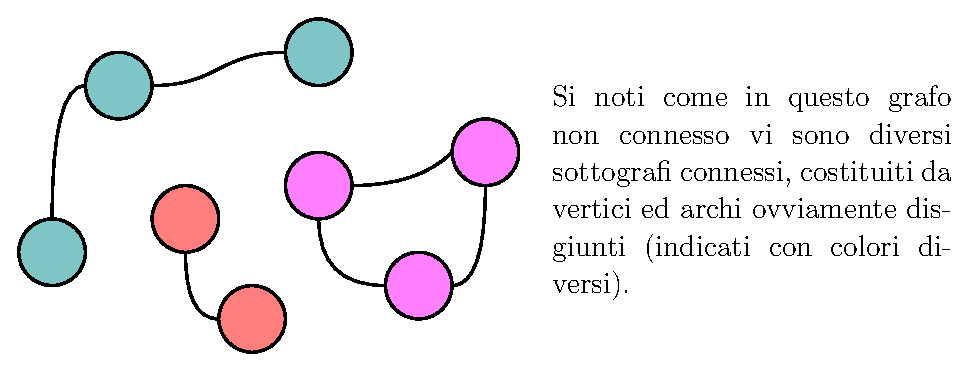
\includegraphics[width=0.9\textwidth ]{images/comp.eps}
\end{center}
Saper riconoscere le componenti di un grafo è un problema noto, che trova applicazione in svariati ambiti, ad esempio,
nell'identificazione delle reti di amicizia in un social network, per capire se ci sono grandi gruppi di persone
per i quali non vi è nemmeno 1 collegamento.\acc
Il problema è il seguente, si vuole scrivere un algoritmo che identifichi tutte le componenti di un grafo,
associando ad ogni vertice, un indice che ne indica la componente, dato un grafo \(G\), e due vertici
\(x,y\), si vuole costruire
un array Comp  tale che : \begin{center}
    Comp[\(x\)]=Comp[\(y\)]\(\iff\)\(x\) ed \(y\) sono nella stessa componente
\end{center}
Utilizziamo la versione ricorsiva del DFS, modificandola a dovere, sono necessarie 2 funzioni : \greybox{
\code{DFSRecComp(graph G, vert x,int[n] Comp, int index)\{}\comm{funzione di supporto}\\
\hphantom{ident}\code{Comp[x]=index}\\
\hphantom{ident}\code{for each y\(\in\)x.adiacenti\{}\comm{per ogni adiacente di x}\\
\hphantom{ident}\hphantom{ident}\code{if(Comp[y]==0)\{}\\
\hphantom{ident}\hphantom{ident}\hphantom{ident}\code{DFSRec(G,y,Comp,index)}\\
\hphantom{ident}\hphantom{ident}\code{\}}\\
\hphantom{ident}\code{\}}\\
\code{\}}}\greybox{
    \code{Comp(graph G)\{}\comm{funzione principale da eseguire}\\
    \hphantom{ident}\code{Comp : int[n] = [0,0\(\dots \)0]}\\
    \hphantom{ident}\code{index = 0}\\
    \hphantom{ident}\code{for each x\(\in\)V(G)\{}\comm{per ogni vertice del grafo}\\
    \hphantom{ident}\hphantom{ident}\code{index++}\\
    \hphantom{ident}\hphantom{ident}\code{DFSRecComp(G,x,Comp,index)}\\
    \hphantom{ident}\code{\}}\\
    \hphantom{ident}\code{return Comp}\\
    \code{\}}}
\subsection{Ordinamento Topologico}\label{OrdTop}
Supponiamo che vi sia un progetto da completare, che viene diviso in \(n\) piccoli processi
\(x_1,x_2\dots x_n\), e supponiamo che fra essi, vi siano delle dipendenze sull'ordine di completamento, ad
esempio : \begin{itemize}
    \item Per essere completato \(x_1\), ha bisogno che siano completati \(x_2,x_3\)
    \item Per essere completato \(x_3\), ha bisogno che sia completato \(x_2\)
\end{itemize}
Dobbiamo pensare ad una programmazione dei processi che rispetti le dipendenze allo scopo di completare il progetto.
Nell'esempio dato, l'ordine corretto sarebbe \(x_2,x_3,x_1\). Utilizziamo un grafo diretto per modellizzare il
problema : i processi saranno i vertici del grafo, e vi sarà un arco da \(x_i\) a \(x_j\) se \(x_i\) dipende
da \(x_j\).\acc In questo modello, una programmazione dei processi non è altro che un ordine dei vertici
del grafo, con la proprietà che tutti i vertici siano orientati "da destra verso sinistra".\begin{center}
    \includegraphics[width=0.3\textwidth ]{images/processiGrafo.eps}
\end{center}
\textbf{Osservazione} : Se in un grafo diretto vi è un ciclo, allora il grafo non ha tutti gli archi che vanno
da destra verso sinistra. \acc
\textbf{Dimostrazione} : Presumiamo che esista tale ordine, allora esiste un vertice \(x\) che è l'ultimo vertice
di tale ordinamento, esiste quindi un arco \((y,x)\) per qualche \(y\), però, nonostante sia l'ultimo,
data la presenza di un ciclo, deve esistere un arco uscente \((x,y)\), ma quindi l'ordine iniziale non è rispettato,
causando una contraddizione. \(\blacksquare\)\acc
Se in un grafo diretto vi è un ciclo, tutto il grafo non ammette la proprietà dell'orientazione degli archi. Tale
proprietà è nota con il nome di \textbf{ordine topologico}, e l'assenza di un ciclo, è condizione necessaria
e sufficiente per garantirla.\acc
\textbf{Proposizione} : Se ogni singolo vertice di un grafo diretto ha almeno un arco uscente, allora
esiste un ciclo.\acc
\textbf{Dimostrazione} : Se esiste sempre un arco uscente, è sempre possibile, partendo da un vertice \(x\) spostarsi
in un suo vertice adiacente, ciò significa che è possibile "camminare" all'infinito sul grafo, il fatto è che il
numero di vertici è finito, quindi prima o poi si visiterà un vertice per una seconda volta, trovandosi in un
ciclo.\begin{center}
    \includegraphics[width=0.7\textwidth ]{images/controEsempio.eps}
\end{center}
\textbf{Corollario} : Se non esiste alcun ciclo in un grafo, allora esiste almeno un vertice che non ha
archi uscenti.\acc
Per ottenere un cosiddetto \textbf{ordinamento topologico}, posso considerare il seguente algoritmo : Si ha un
grafo diretto \(G\), sprovvisto di cicli, si sceglie un qualsiasi vertice privo di archi uscenti, si inserisce
in una lista per poi eliminarlo dal grafo (insieme a tutti i suoi archi associati), dopo ciò, si
ri-esegue l'operazione, inserendo ogni volta il vertice nella prima posizione della lista.\acc Tale algoritmo risulta
parecchio utile, si pensi all'ordinamento topologico applicato al grafo di serializzazione nell'ambito
del controllo della concorrenza
(trattato nel corso di \href{https://github.com/CasuFrost/University_notes/blob/main/Secondo%20Anno/Primo%20Semestre/Basi%20di%20Dati%201/Latex%20source%20file/Basi%20di%20Dati%20modulo%201.pdf}{Basi di Dati 1}).
\greybox{
    \code{OrdinamentoTopologico(graph G)\{}\comm{il grafo è diretto}\\
    \hphantom{ident}\code{L : list}\comm{una lista vuota, sarà l'output dell'algoritmo}\\
    \hphantom{ident}\code{while(G\(\ne\emptyset\))\{}\\
    \hphantom{ident}\hphantom{ident}\code{x=v\(\in\)V(G)|v.adiacentiOut=\(\emptyset\)}\comm{un vertice senza archi uscenti}\\
    \hphantom{ident}\hphantom{ident}\code{L.insert(x)}\\
    \hphantom{ident}\hphantom{ident}\code{G.delete(x)}\\
    \hphantom{ident}\code{\}}\\
    \hphantom{ident}\code{return L}\\
    \code{\}}}\begin{center}
    \includegraphics[width=1\textwidth ]{images/ordTopologico.eps}
\end{center}
Il \textit{problema} di questo algoritmo è il suo costo computazionale, di fatto è troppo dispendioso : Per
controllare se un vertice non ha archi uscenti, si è in \(O(n)\), inoltre il ciclo \code{while} controlla
tutti i vertici, quindi si è nuovamente in \(O(n)\).    \acc  La cancellazione di un vertice risulta dispendiosa, in
quanto bisona eliminare anche tutti gli archi associati, ossia, eliminare il vertice da tutte le liste
di adiacenza degli altri vertici, il numero di controlli dipende dal grado di ogni vertice,
quindi costa \(O(m)\). In totale, l'intero algoritmo ha una complessità \(O(n\cdot(n+m))\), vorremmo riuscire
ad ottenere lo stesso output in tempo lineare.
\subsubsection{Contatore nel DFS e Relazioni sull'Arborescenza}
Vogliamo considerare un estensione del normale DFS, consideriamo un contatore, denotato \code{cc}, tale contatore,
verrà incrementato ogni qual volta verrà visitato per la prima volta un nuovo nodo.\acc Consideriamo inoltre, due nuove
funzioni \(t:V(G)\rightarrow\mathbb{N}\) e \(T:V(G)\rightarrow\mathbb{N}\), sia \(v\) un vertice, \(t(v)\) sarà uguale al valore
del contatore \code{cc} nel momento in cui \(v\) viene visitato per la prima volta, invece \(T(v)\) sarà uguale al valore
del contatore \code{cc} nel momento in cui \(v\) viene visitato per l'ultima volta, ossia quando esso viene rimosso dallo stack.\acc
\textbf{Osservazione} : \begin{itemize}
    \item Per ogni coppia di vertici \(v,u\), si ha che \(t(v)\ne t(u)\)
    \item Per ogni vertice \(v\), si ha che \(t(v)\le T(V)\)
    \item Sia \(v\) un vertice, se \(t(v)=T(V)\), allora \(v\), è una foglia nell'albero di visita derivante dall'applicazione
          del DFS.
    \item Sia \(n\) il numero di vertici e \(v_0\) la radice dell'albero di visita, si ha che \(t(v_0)=1\land T(v_0)=n\).
\end{itemize}
Esempio di applicazione dell'algoritmo (si parte dal vertice \(1\)) : \begin{center}
    \includegraphics[width=1.05\textwidth ]{images/dfsContatore.eps}
\end{center}
Ad ogni vertice \(v\), è associato un \textit{intervallo} \([t(v),T(v)]\), gli intervalli di vertici diversi possono
essere confrontati, e si ricade sempre in uno dei seguenti casi.\acc
\textbf{Osservazione} : Siano \(v\) e \(u\) due vertici distinti del grafo, uno dei seguenti punti è sempre vero:\begin{itemize}
    \item \(i)\) $[t(v),T(v)]\subseteq[t(u),T(u)]$
    \item \(ii)\) $[t(v),T(v)]\supseteq[t(u),T(u)]$
    \item \(iii)\) $[t(v),T(v)]\cap[t(u),T(u)]=\emptyset$
\end{itemize}
\textbf{Dimostrazione} : Il quarto ed ultimo caso possibile, sarebbe un intersezione del tipo: $$
    t(u)<t(v)\le T(u)<t(v)$$ Basta dimostrare che questa casistica non può verificarsi. Se \(u\) è stato inserito
nello stack prima di \(v\), si avrà che \(T(u)\ge t(v)\), questo implica che \(u\) era già nello stack quando
\(v\) è stato inserito, ma allora è impossibile togliere \(u\) prima di \(v\), e necessariamente \(T(u)>T(v)\). \(\blacksquare\)\acc
Adesso, consideriamo il grafo sulla quale è stato applicato il nuovo DFS con contatore, e consideriamo gli archi che \textit{non appartengono}
all'arborescenza, ossia gli archi che non sono stati attraversati durante il DFS (nell'immagine esplicativa precedente, quelli colorati in
azzurro). \acc
Vi è un fatto interessante, consideriamo tutti un qualsiasi arco non facente parte dell'arborescenza, esso indica due vertici \((v,u)\),
e tali vertici posseggono gli intervalli che possono essere messi in relazione, ricadendo in uno dei 3 casi prima citati.\acc Gli archi
non facenti parte dell'arborescenza, se considerati nell'arborescenza, potranno essere di 3 tipi, o partire da un vertice ed andare
verso un suo antenato, o partire da un vertice ed andare
verso un suo successore, oppure attraversare due vertici di due diramazioni differenti, in effetti, riguardo la relazione
di intervalli prima citata, si ha che : \begin{itemize}
    \item Se i due vertici dell'arco ricadono nel punto \((i)\), allora l'arco va da un antenato ad un discendente (\textbf{arco in avanti}).
    \item Se i due vertici dell'arco ricadono nel punto \((ii)\), allora l'arco va da un discendente ad un antenato  (\textbf{arco all'indietro}).
    \item Se i due vertici dell'arco ricadono nel punto \((iii)\), allora l'arco attraversa due diramazioni differenti  (\textbf{arco di attraversamento}).
\end{itemize}
Riguardo il grafo del precedente esempio : \begin{center}
    \includegraphics[width=1.05\textwidth ]{images/archiArborescenza.eps}
\end{center}
Si noti come l'arco che va dal vertice 8 al vertice 9, è un \textit{arco all'indietro}, infatti gli intervalli dei due
vertici ricadono nel secondo caso : \([9,9]\supseteq[7,9]\).\acc
Si noti come l'arco che va dal vertice 2 al vertice 4, è un \textit{arco in avanti}, infatti gli intervalli dei due
vertici ricadono nel primo caso : \([2,6]\subseteq[6,6]\).\acc
Si noti come l'arco che va dal vertice 7 al vertice 5, è un \textit{arco di attraversamento}, infatti gli intervalli dei due
vertici ricadono nel terzo caso : \([8,9]\cap[4,5]=\emptyset\).\acc
Se dovessi applicare lo stesso algoritmo ai grafi non diretti, non si potrebbe definire una relazione di antenato-discendente,
in quanto ogni arco è percorribile per entrambe le direzioni, quindi i casi \((i)\) e \((ii)\) indicherebbero la stessa
situazione.\acc
Inoltre, è impossibile che, per due nodi \(u,v\) si verifichi che $[t(v),T(v)]\cap[t(u),T(u)]=\emptyset$, quindi
il caso \((iii)\) è impossibile. Si vuole dare ora lo pseudocodice di una modifica del DFS, che restituisca in output 3 liste, conteneti
gli archi in avanti, all'indietro, e di attraversamento.\greybox{
\code{DFSconArchi(graph G, vert x,)\{}\comm{il grafo è diretto}\\
\hphantom{ident}\code{int cc=1}\\
\hphantom{ident}\code{t : int[n]} \comm{array lungo \(n\) inizializzato a zero}\\
\hphantom{ident}\code{T : int[n]}\comm{array lungo \(n\) inizializzato a zero}\\
\hphantom{ident}\code{t[x]=1}\\
\hphantom{ident}\code{T[x]=|V(G)|}\\
\hphantom{ident}\code{S : stack = \{x\}}\\
\hphantom{ident}\code{Vis : int[n] = [0,0\(\dots \)0]}\\
\hphantom{ident}\code{Vis[x]=1}\\
\hphantom{ident}\code{while(S\(\ne\emptyset\))\{}\\
\hphantom{ident}\hphantom{ident}\code{y=S.top()}\\
\hphantom{ident}\hphantom{ident}\code{if(\(\exists z|(y,z)\in E(G)\land \) Vis[z]==0)\{}\comm{l'arco ha la giusta orientazione}\\
\hphantom{ident}\hphantom{ident}\hphantom{ident}\code{S.push(z)}\\
\hphantom{ident}\hphantom{ident}\hphantom{ident}\code{c++}\\
\hphantom{ident}\hphantom{ident}\hphantom{ident}\code{t[z]=cc}\\
\hphantom{ident}\hphantom{ident}\hphantom{ident}\code{Vis[z]=1}\\
\hphantom{ident}\hphantom{ident}\code{\}}\\
\hphantom{ident}\hphantom{ident}\code{else\{}\\
\hphantom{ident}\hphantom{ident}\hphantom{ident}\code{S.pop()}\\
\hphantom{ident}\hphantom{ident}\hphantom{ident}\code{T[z]=cc}\\
\hphantom{ident}\hphantom{ident}\code{\}}\\
\hphantom{ident}\code{\}}\\
\hphantom{ident}\code{A : graph = arborescenza generata dal DFS}\\
\hphantom{ident}\code{A' : graph = G-A}\comm{il complementare dell'arborescenza}\\
\hphantom{ident}\code{av : list}\\
\hphantom{ident}\code{ind : list}\\
\hphantom{ident}\code{att : list}\\
\hphantom{ident}\code{for each (x,y)\(\in\)E(A')\{}\\
\hphantom{ident}\hphantom{ident}\code{switch(t[x],T[x],t[y],T[y])\{}\\
\hphantom{ident}\hphantom{ident}\hphantom{ident}\code{$[t(v),T(v)]\subseteq[t(u),T(u)]$ : sv.append((x,y))}\comm{primo caso}\\
\hphantom{ident}\hphantom{ident}\hphantom{ident}\code{$[t(v),T(v)]\supseteq[t(u),T(u)]$ : ind.append((x,y))}\comm{secondo caso}\\
\hphantom{ident}\hphantom{ident}\hphantom{ident}\code{$[t(v),T(v)]\cap[t(u),T(u)]=\emptyset$ : att.append((x,y))}\comm{terzo caso}\\
\hphantom{ident}\hphantom{ident}\code{\}}\\
\hphantom{ident}\code{\}}\\
\hphantom{ident}\code{return av,ind,att}\\
\code{\}}}\newpage
La domanda da porsi adesso è, la presenza di questi archi \textit{in avanti}, \textit{indietro} e di \textit{attraversamento},
quali informazioni fornisce riguardo le proprietà del grafo?\acc Consideriamo un grafo \(G\) non diretto e connesso, vuol dire che per
ogni coppia di vertici \(x\) ed $y$ esiste un cammino da $x$ ad $y$, se dovesse esistere un'arco \((x,y)\in E(G)\), allora
vi sarà un ciclo.\acc
\textbf{Proposizione} : Sia \(G\) un grafo connesso non diretto, se esiste un ciclo, allora, per una
\textit{qualsiasi applicazione} del DFS, esisterà un arco all'indietro (che è identico all'arco in avanti,
essendo il grafo non diretto).\acc
\textbf{Dimostrazione} : Se in \(G\) c'è un ciclo, allora esisterà un arco che non sarà presente nell'albero di visita
generato dal DFS (essendo un albero, non ha cicli), quindi esiste un arco esterno a tale albero che collega due nodi,
ed è necessariamente un arco all'indietro. \(\blacksquare\)
\begin{center}
    \textit{Conclusione} : DFS genera arco all'indietro $\iff$ \(G\) ha un ciclo
\end{center}
Consideriamo ora il caso in cui il grafo è diretto, sia \(v\) un vertice, ed \(u\) un suo discendente nell'arborescenza
generata da una qualsiasi applicazione del DFS, esiste un cammino diretto da \(v\) ad \(u\).\begin{center}
    \includegraphics[width=0.5\textwidth ]{images/discentente.eps}
\end{center}
Se \(u\) è un discendente di \(v\), allora \(u\) è stato visitato la prima volta dopo di \(v\), allora è stato
rimosso dallo stack prima di \(v\) $$t(v)<t(u)\le T(u)\le T(v)$$
Se esistesse un arco $(u,v)$, allora sarebbe un arco all'indietro. Sappiamo che per ogni coppia di vertici
\(u,v\), se \(u\) è un discendente di \(v\), allora esiste un cammino diretto da \(v\) ad \(u\) nell'arborescenza.\acc
\textbf{Osservazione} : Se esistesse un arco all'indietro nell'arborescenza generata dal DFS, allora
il grafo avrebbe un ciclo.\acc
\textbf{Proposizione 1} : Se \(G\) è un grado diretto, e tutti i suoi vertici sono raggiungibili da un
vertice di partenza \(x\), allor, una qualsiasi applicazione del DFS partendo da \(x\) genera un
arco all'indietro nell'arborescenza \textit{se e solo se} esiste un ciclo in \(G\).\acc
Assumendo che in \(G\) ci sia un ciclo, consideriamo i vertici che compongono il ciclo :
$c_0,c_1,c_2\dots,c_k$, elencati in ordine di visita nel DFS, quindi \(c_0\) è il primo vertice del ciclo
visitato durante una qualsiasi applicazione del DFS.
\acc\textbf{Proposizione 2} : Tutti i vertici del ciclo (escluso $c_0$), verranno visitati per la prima
volta \textit{prima} che \(c_0\) venga rimosso dallo stack.\acc
\textbf{Dimostrazione della prop. 2} : So che $\forall i\in\{1\dots k\},t(c_i)>t(c_0)$, assumiamo che
esista un \(c_i\) fissato che non rispetti la condizione della proposizione, ossia $$t(c_i)>T(c_0)$$
Tale $c_i$ potrebbe non essere l'unico, sia però il vertice visitato per primo fra quelli che non rispettano
la condizione, considero ora il vertice visitato appena prima di $c_i$, ossia $c_{i-1}$, so che
$t(c_{i-1})>t(c_0)$ e che $t(c_{i-1})\le T(c_0)$, ovviamente non può essere superiore perchè il primo
vertice che viola la condizione, è il suo successivo $c_i$. Si verifica la condizione :
\begin{center}
    \includegraphics[width=1\textwidth ]{images/realLine.eps}
\end{center}
Sappiamo però che $c_{i-1}$ viene prima di $c_i$ nel ciclo, esiste quindi un arco $(c_{i-1},c_i)$, quindi
è impossibile che $c_{i-1}$ venga rimosso dallo stack prima di $c_i$, è quindi una contraddizione, e
necessariamente la proposizione è vera. \(\blacksquare\)\acc
\textbf{Dimostrazione della prop. 1} : Data la \textit{proposizione 2}, necessariamente l'arco del
ciclo \((c_k,c_0)\) è un arco all'indietro. \begin{center}
    \includegraphics[width=1\textwidth ]{images/realLine2.eps}
\end{center}\subsubsection{Pozzo Universale}
Si consideri ora un vertice $x$ di un generico grafo diretto $G$, che rispetti le seguenti proprietà : \begin{itemize}
    \item $\forall y\in V(G), \nexists (x,y)\in E(G)$
    \item $\forall y\in V(G), \exists (y,x)\in E(G)$
\end{itemize}
È un vertice che non ha archi uscenti, e tutti gli altri vertici del grafo hanno un arco che diretto verso di esso,
tale vertice prende il nome di \textit{pozzo universale}.\begin{center}
    \includegraphics[width=0.6\textwidth ]{images/pozzo.eps}
\end{center}
\textit{Esercizio} : Si dia lo pseudocodice di un algoritmo che in $O(n)$, dove $n$ è il numero di vertici,
stabilisca se il grafo in input ha o non ha un pozzo universale, il grafo è dato sottoforma di matrice di
adiacenza.\acc
La costrizione più grande è la richiesta del costo computazionale, è chiaro che non è possibile
controllare ogni vertice in maniera dettagliata, vedendo se è o non è un pozzo universale in base
ai valori che assumono le entrate nella matrice.\acc
Una possibile idea è di controllare in coppia tutti i vertici, escludendo i possibili che sicuramente non sono
un pozzo universale : Si comincia controllando due vertici a caso \(x,y\), se l'entrata della matrice
$m(x,y)$ è 1, vuol dire che esiste un arco che va da $x$ ad $y$, dovremmo quindi escludere $x$ dato che ha
archi uscenti, e continuare con $y$, altrimenti continueremo con $x$.\acc
Alla fine, avremo un vertice candidato ad essere un pozzo, e controlleremo in maniera esplicita se lo è o no.
\greybox{
    \code{PozzoUniversale(m)\{}\comm{l'input è la matrice di adiacenza}\\
    \hphantom{ident}\code{candidato = 1}\\
    \hphantom{ident}\code{n = m[1].length()}\comm{n è il numero di vertici}\\
    \hphantom{ident}\code{for(i=2;i\(\le\)n;i++)\{}\\
    \hphantom{ident}\hphantom{ident}\code{if(m[candidato,i]==1)\{}\\
    \hphantom{ident}\hphantom{ident}\hphantom{ident}\code{candidato=i}\\
    \hphantom{ident}\hphantom{ident}\code{\}}\\
    \hphantom{ident}\code{\}}\\
    \hphantom{ident}\code{for(i=1;i\(\le\)n;i++)\{}\\
    \hphantom{ident}\hphantom{ident}\code{if(m[candidato,i]==1)\{}\\
    \hphantom{ident}\hphantom{ident}\hphantom{ident}\code{return false}\comm{il candidato ha un arco uscente}\\
    \hphantom{ident}\hphantom{ident}\code{\}}\\
    \hphantom{ident}\code{\}}\\
    \hphantom{ident}\code{for(i=1;i\(\le\)n;i++)\{}\\
    \hphantom{ident}\hphantom{ident}\code{if(m[i,candidato]==0 \(\land\) i\(\ne\)candidato)\{}\\
    \hphantom{ident}\hphantom{ident}\hphantom{ident}\code{return false}\comm{un nodo non ha un arco verso il candidato}\\
    \hphantom{ident}\hphantom{ident}\code{\}}\\
    \hphantom{ident}\code{\}}\\
    \hphantom{ident}\code{return true}\\
    \code{\}}}
\subsubsection{Ordine Topologico in Tempo Lineare}
Tornando al DFS con il contatore, esiste ovviamente anche una versione ricorsiva, composta da due funzioni,
una "globale" che inizializza il processo, ed una ricorsiva che opera.\greybox{
    \code{DFSglobal(G,x)\{}\\
    \hphantom{ident}\code{Vis : int[n] = [0,0...,0]}\\
    \hphantom{ident}\code{t : int[n] = [0,0...,0]}\\
    \hphantom{ident}\code{T : int[n] = [0,0...,0]}\\
    \hphantom{ident}\code{c : int = 1}\\
    \hphantom{ident}\code{DFSrecursive(x,Vis,c,t,T)}\comm{prima chiamata della funzione ricorsiva}\\
    \hphantom{ident}\code{return Vis}\\
    \code{\}}}
L'algoritmo rimane in $O(n+m)$, passiamo ora alla funzione ricorsiva.\greybox{
    \code{DFSrecursive(x,Vis,c,t,T)\{}\\
    \hphantom{ident}\code{while($\exists$y$\in$V(G) | Vis[y]=0 $\land$ (x,y)$\in$E(G))\{}\\
    \hphantom{ident}\hphantom{ident}\code{Vis[y]=1}\\
    \hphantom{ident}\hphantom{ident}\code{c++}\\
    \hphantom{ident}\hphantom{ident}\code{t[y]=c}\\
    \hphantom{ident}\hphantom{ident}\code{DFSrecursive(y,Vis,c,t,T)}\\
    \hphantom{ident}\code{\}}\\
    \hphantom{ident}\code{T[x]=c}\\
    \code{\}}}
\textbf{Proposizione} : Per ogni arco $(v,u)$ in un grafo diretto, si ha che $t(u)\le T(v)$.\acc
\textbf{Dimostrazione} : Se così non fosse, vorrebbe dire che $t(u)>T(v)$, significherebbe che avremmo
chiuso (tolto dallo stack) $v$ quando vi era ancora possibilità di continuare su $u$, quindi
è impossibile che ciò accada. $\blacksquare$\acc
Torniamo adesso all'\textit{ordinamento topologico}, nei capitoli precedenti, si è visto che, se il grafo
è ciclico allora esistono degli archi all'indietro. In caso contrario, ci sono due restanti possibilità
per ogni arco $(v,u)$ :\begin{itemize}
    \item \(ii)\) $[t(v),T(v)]\supseteq[t(u),T(u)]$
    \item \(iii)\) $[t(v),T(v)]\cap[t(u),T(u)]=\emptyset$
\end{itemize}
Sicuramente $t(u)\le T(u)\le T(v)$, $t(v)$ può trovarsi in uno dei due seguenti intervalli :\begin{center}
    \includegraphics[width=0.8\textwidth ]{images/cases.eps}
\end{center}
Il fatto, è che $T(u)\le T(v)$, e ciò vale per ogni arco del grafo $(v,u)$, nel corrispettivo ordine
topologico in cui tutti gli archi andranno da "sinistra verso destra", si avrà che, seguento quest'ordine,
i valori di $T$ per i vertici coinvolti saranno \textit{decrescenti}.\begin{center}
    \includegraphics[width=0.7\textwidth ]{images/t_T_crescenza.eps}
\end{center} La dove si causerà una situazione
di "tie break", ossia in cui i valori di $T$ sono coincidenti per due vertici, si avrà che essi differiranno
per i valori di $t$, che secondo l'ordine prima menzionato saranno strettamente crescenti, nel risultante
ordine topologico, i vertici chiusi (tolti dallo stack) per ultimi, saranno quelli a sinistra.\greybox{
    \code{ORDtopologico(G)\{}\comm{funzione globale}\\
    \hphantom{ident}\code{L : list}\comm{l'output, conterrà i vertici dell'ordine topologico}\\
    \hphantom{ident}\code{Vis : int[n] = [0,0...,0]}\\
    \hphantom{ident}\code{for each (v$\in$V(G))\{}\\
    \hphantom{ident}\hphantom{ident}\code{if(Vis[v]==0)\{}\\
    \hphantom{ident}\hphantom{ident}\hphantom{ident}\code{DFSord(G,v,Vis,L)}\\
    \hphantom{ident}\hphantom{ident}\code{\}}\\
    \hphantom{ident}\code{\}}\\
    \code{\}}}\greybox{
    \code{DFSord(G,v,Vis,L)\{}\comm{funzione ricorsiva}\\
    \hphantom{ident}\code{Vis[v]=1}\\
    \hphantom{ident}\code{for each (w adiacente di v)\{}\\
    \hphantom{ident}\hphantom{ident}\code{if(Vis[w]==0)\{}\\
    \hphantom{ident}\hphantom{ident}\hphantom{ident}\code{DFSord(G,w,Vis,L)}\\
    \hphantom{ident}\hphantom{ident}\code{\}}\\
    \hphantom{ident}\code{\}}\\
    \hphantom{ident}\code{L.insert(v,0)}\comm{inserisci il vertice nella prima posizione della lista}\\
    \code{\}}}
\subsection{Ponti sui Grafi non Diretti}\label{PontiGrafiNonDir}
\hphantom{a}
\begin{center}
    \includegraphics[width=0.7\textwidth ]{images/ponte.eps}
\end{center}
Come si può procedere per verificare che un arco $(u,v)$ sia o no un ponte? Posso rimuovere l'arco, e controllare con il DFS
se esiste ancora un cammino fra i due vertici coinvolti, se esiste, allora quell'arco non era un ponte. Se volessi trovare
tutti i ponti di un grafo, questa operazione risulterebbe poco efficiente, e l'algoritmo avrebbe complessità $O(m\cdot(n+m))$.\acc
\textbf{Osservazione} : Qualsiasi arco coinvolto in un ciclo, non è un ponte, viceversa, se un arco è un ponte, allora
non fa parte di un ciclo.\acc
Ne consegue che, qualsiasi arco che non fa parte dell'albero di visita derivante da una qualsiasi applicazione del DFS
(gli archi all'indietro), sicuramente non è un ponte. Quindi un ponte fa parte dell'albero di visita, non è necessario
controllare tutti gli archi. Si considerino i due seguenti alberi di visita di due grafi che
differiscono esclusivamente per un arco.\begin{center}
    \includegraphics[width=1\textwidth ]{images/checkPonte.eps}
\end{center}
Osservando la seguente immagine, si noti che, l'arco viola del primo grafo, è un ponte, invece l'arco viola del
secondo grafo, non lo è, rimane infatti connesso grazie all'arco arancione, che non fa parte dell'albero di
visita, da tali considerazioni, si giunge alla seguente proposizione.\acc
\textbf{Proposizione} : Sia $T$ un albero di visita derivante da una qualsiasi applicazione del DFS su un
grafo connesso e non diretto, e sia $(u,v)\in E(T)$, un arco dell'albero, dove $v$ è il padre di $u$, si ha che,
l'arco  $(u,v)$ è un ponte \textit{se e solo se} non esiste alcun arco all'indietro da un qualsiasi vertice
discendente di $u$, ad un qualsiasi vertice antenato di $v$ ($v$ compreso).\acc
\textbf{Dimostrazione} : \boxedMath{$(1)\implies(2)$} Sia $T_u$ l'insieme dei discendenti di $u$. Se esistesse un arco da  $T_u$ all'indietro,
allora $(u,v)$ sarebbe parte di un ciclo, e sicuramente non sarebbe un ponte. \boxedMath{$(2)\implies(1)$} Assumiamo che
$(u,v)$ non sia un ponte, allora esiste un cammino $u\rightarrow v$ che non fa uso dell'arco in questione. Esiste sicuramente
un punto nel cammino, in cui si passa da un vertice $x$ tale che $x\notin T_u$, ad un vertice $y$ tale che
$y\in T_u$, ma sappiamo che non esistono archi all'indietro, ciò porta ad una contraddizione. $\blacksquare$\acc
Scriviamo adesso lo pseudocodice di un algoritmo che restituisce tutti i ponti di un grafo in tempo lineare, come prima, diamo
la definizione di \textit{punto di back}, o semplicemente \textit{back}.\acc
\textbf{Definizione} : Il \textit{back} di un vertice $u$ in un albero di visita, non è altro che il vertice più
vicino alla radice che è possibile raggiungere con un arco da $u$ o da uno dei suoi discendenti.\begin{center}
    \includegraphics[width=1\textwidth ]{images/back.eps}
\end{center}
Vogliamo quindi un algoritmo che, per un arco $(u,v)$, dove $v$ è il padre di $u$, si controlli il
back di $u$, se esso è presente fra $v$ ed i suoi antenati, allora l'arco non è un ponte, altrimenti lo è.
\greybox{
    \code{Ponti(G : grafo connesso non diretto)\{}\comm{funzione globale}\\
    \hphantom{ident}\code{t : int[n] = [0,0...,0]}\\
    \hphantom{ident}\code{c : int = 0}\\
    \hphantom{ident}\code{Ponti : list}\comm{l'output}\\
    \hphantom{ident}\code{z = un vertice a caso di G}\\
    \hphantom{ident}\code{DFSponte(G,z,z,t,c,Ponti)}\\
    \hphantom{ident}\code{return Ponti}\\
    \code{\}}}\greybox{
\code{DFSponte(G, v, z, t, c, Ponti)\{}\comm{funzione ricorsiva, z è il padre di v}\\
\hphantom{ident}\code{back=t[v]}\\
\hphantom{ident}\code{c++}\\
\hphantom{ident}\code{t[v]=c}\\
\hphantom{ident}\code{for each (w adiacente di v)\{}\\
\hphantom{ident}\hphantom{ident}\code{if(t[w]==0)\{}\\
\hphantom{ident}\hphantom{ident}\hphantom{ident}\code{b=DFSponte(G,w,v,t,c,Ponti)}\\
\hphantom{ident}\hphantom{ident}\hphantom{ident}\code{back = min(b,back)}\\
\hphantom{ident}\hphantom{ident}\code{\}}\\
\hphantom{ident}\hphantom{ident}\code{else if(w$\ne$z)\{}\\
\hphantom{ident}\hphantom{ident}\hphantom{ident}\code{back = min(t[w],back)}\\
\hphantom{ident}\hphantom{ident}\code{\}}\\
\hphantom{ident}\code{\}}\\
\hphantom{ident}\code{if(back==t[v])\{}\\
\hphantom{ident}\hphantom{ident}\code{Ponti.add((v,z))}\\
\hphantom{ident}\code{\}}\\
\hphantom{ident}\code{return back}\\
\code{\}}}
\subsection{Componenti Fortemente Connesse}
Abbiamo già dato la definizione di fortemente connesso per un grafo diretto, ossia un grafo $G$ di cui,
per ogni coppia di vertici $(u,v)$ esiste un cammino da $u$ a $v$ e viceversa. Quando un grafo è non diretto, risulta
facile trovare le componenti connesse, in quanto è facilmente visualizzabile come un "pezzo" di grafo connesso
distaccato dal resto.\acc
In un grafo diretto, una componente è un sottografo fortemente connesso \textit{massimale}, ossia, che non è contenuto in
un sottografo più grande fortemente connesso.\acc
\textbf{Osservazione} : Ogni vertice di un grafo diretto è contenuto in un componente fortemente connesso, dato che
al minimo esiste il componente costituito dall'unico vertice.\acc
\textbf{Osservazione} : Non esistono più componenti che hanno vertici in comune, ogni vertice appartiene ad un solo
componente.\begin{center}
    \includegraphics[width=0.7\textwidth ]{images/compoGrafDir.eps}
\end{center}
Si vuole un algoritmo capace di trovare le componenti fortemente connesse di un grafo diretto.
\subsubsection{Contrazione di Vertici}
\textbf{Definizione} : Sia $G$ un grafo diretto, e sia $H\in V(G)$ un insieme di vertici, è possibile
\textit{contrarre} i vertici, facendoli "collassare" in un unico vertice, ottenendo il grafo $G$ contratto $H$, denotato
$\nicefrac{G}{H}$. Si denota con $V_H$ il nuovo vertice contratto.\begin{itemize}
    \item  $V(\nicefrac{G}{H}) := (V(G)\backslash H)\cup \{V_H\}$
    \item $E(\nicefrac{G}{H}) := \{(x,y)\in E(G)| x,y\notin H\}\cup$\\
          \hphantom{identaiden.}$\{(w,V_H)\text{ se } \exists(w,y)|w \notin V_H\land y \in V_H\}\cup$\\
          \hphantom{identaiden.}$\{(V_H,w)\text{ se } \exists(y,w)|w \notin V_H\land y \in V_H\}$
\end{itemize} \begin{center}
    \includegraphics[width=0.55\textwidth ]{images/contrazione.eps}
\end{center}
\textbf{Proposizione} : Se $G$ è un grafo fortemente connesso ed $H$ è un sottografo connesso, allora $\nicefrac{G}{H}$ è
ancora un grafo fortemente connesso.\begin{center}
    \includegraphics[width=0.65\textwidth ]{images/propFortCOnn.eps}
\end{center}
\textbf{Dimostrazione} : Nel grafo
originale $G$ esiste un cammino $P$ da un qualsiasi nodo $x$ ad un qualsiasi nodo contenuto in $H$, ed esiste un
cammino $Q$ da un qualsiasi nodo in $H$ ad un qualsiasi nodo $x$, siano questi cammini quelli più corti possibile, essi
per definizione di $\nicefrac{G}{H}$ saranno anche in $\nicefrac{G}{H}$, quindi esisterà un cammino da
da $x$ a $V_H$ e da $V_H$ ad $x$, quindi il grafo $\nicefrac{G}{H}$ è fortemente connesso. $\blacksquare$
\subsubsection{C-radice di un Componente Fortemente Connesso}
\textbf{Osservazione} : Se $G$ è fortemente connesso e non è banale, allora contiene sicuramente un ciclo, quindi esiste un
arco $(x,y)$ per cui esiste anche un cammino da $y$ ad $x$, che insieme all'arco precedente compone il ciclo. Un ciclo inoltre
è un sottografo fortemente connesso, se applichiamo la contrazione ricorsivamente sui cicli, otterremo le componenti connesse.
\acc
Se $u_1,u_2\dots,u_k$ sono fortemente connessi in $\nicefrac{G}{C}$, con
$C$ un insieme e $V_C$ il vertice contratto, si ha che le componenti in
$G$ sono $u'_1,u'_2\dots,u'_k$ con:$$
    u'_i=\begin{cases}
        u_i\text{ se }V_C\notin u_i \\
        (u_i\backslash \{V_C\})\cup \{V(C)\}\text{ se }V_C\in u_i
    \end{cases}
$$ Se il grafo non ha cicli, ogni vertice è un componente connesso. Vediamo
ora l'algoritmo non lineare.\greybox{
    \code{Fort(G graph)\{}\acc
    \hphantom{ident}\code{C = un ciclo in G}\\
    \hphantom{ident}\code{if (C non esiste)\{}\comm{non ci sono cicli nel grafo}\\
    \hphantom{ident}\hphantom{ident}\code{return \{\{v\}|v $\in$ V(G)\}}\\
    \hphantom{ident}\code{\}}\\
    \hphantom{ident}\code{G=$\nicefrac{G}{C}$}\\
    \hphantom{ident}\code{$V_C$ = vertice contratto}\\
    \hphantom{ident}\code{($u_1,u_2\dots,u_k$)=Fort(G)}\\
    \hphantom{ident}\code{for (i in 1...k)\{}\\
    \hphantom{ident}\hphantom{ident}\code{if ($V_C\notin u_i$)\{}\\
    \hphantom{ident}\hphantom{ident}\hphantom{ident}\code{$u'_i=u_i$}\\
    \hphantom{ident}\hphantom{ident}\code{\}}\\
    \hphantom{ident}\hphantom{ident}\code{else \{}\\
    \hphantom{ident}\hphantom{ident}\hphantom{ident}\code{$u'_i=(u_i\backslash V_C)\cup \{V(C)\}$}\\
    \hphantom{ident}\hphantom{ident}\code{\}}\\
    \hphantom{ident}\code{\}}\\
    \hphantom{ident}\code{return ($u'_1,u'_2\dots,u'_k$)}\\
    \code{\}}}
Tale algoritmo ha complessità $O(n\cdot(n+m))$, voglio modificare il DFS per ottenere lo stesso algoritmo che operi in
tempo lineare.\acc
\textbf{Definizione} : Data l'esecuzione del DFS su un grafo $G$ diretto, e dato un componente fortemente
connesso $C$ del grafo, una \textbf{C-radice} è il primo vertice appartenente a $C$, visitato nel DFS.\acc
\textbf{Proposizione} : Sia $T$ un arborescenza di visita di un DFS, e sia $T(u)$ l'insieme dei discendenti di un nodo
$u$, sia poi $C(u)$ il componente fortemente connesso nella quale è contenuto $u$, valgono le seguenti:\begin{enumerate}
    \item $C(u)\subseteq T(u)$
    \item Se $u_1,u_2\dots,u_k$ sono le C-radici in $T(u)$, si ha che $\displaystyle T(u)=\bigcup_{i=1}^k C(u_i)$
\end{enumerate}
\textbf{Dimostrazione} \boxedMath{1} Assumiamo che $C(u)\nsubseteq  T(u)$, allora esiste un arco $(x,y)\in C(u)$ tale
che $x\in T(u)\land y\notin T(u)$, tale arco è, o all'indietro, o di attraversamento. In entrambi i casi, si ha che
$y$ è un antenato di $u$ $\implies$ $y$ è stato visitato per la prima volta, prima di $u$ $\implies$ $u$ non è la
C-radice del suo componente, ma per ipotesi $u$ è la C-radice, si ha quindi una contraddizione.\acc
\boxedMath{2} Se $u_i\in T(u)$, per il punto (1), $C(u_i)\subseteq T(u_i) \subseteq T(u)\implies C(u_i)\subset T(u)$. Dimostro
adesso che,
se $w\in T(u)$, il componente $C(w)$ non ha elementi al di fuori di $T(u)$. Assumiamo per assurdo che ciò sia falso, si ha
che $C(w)\nsubseteq T(u)$, sia allora $z$ la C-radice di $C(w)$, si ha che  \begin{itemize}
    \item $w$ è un discendente di $z$
    \item $u$ è un discendente di $z$
\end{itemize}
Ma allore esistono i cammini da $z$ ad $u$, e da $u$ a $w$, ma so che nel componente fortemente connesso $C(w)$ esiste
un cammino da $w$ a $z$, ma allora $u,w,z\in C(w)$, ma inizialmente si è detto che $u$ è la C-radice, ma come può esserlo se
$u$ è un discendente di $z$? C'è una contraddizione, quindi $C(w)\subseteq T(u)$. $\blacksquare$
\greybox{
    \code{DFS\_Scc(G : graph, v : vert, C : stack, Output : list)\{}\comm{ricorsiva}\\
    \hphantom{ident}\code{segna v come visitato}\\
    \hphantom{ident}\code{C.push(v)}\\
    \hphantom{ident}\code{for each (u adiacente a v $\land$ u non ancora visitato)\{}\\
    \hphantom{ident}\hphantom{ident}\code{DFS\_Scc(G,u,C,Output)}\\
    \hphantom{ident}\code{\}}\\
    \hphantom{ident}\code{if(v è una C-radice)\{}\\
    \hphantom{ident}\hphantom{ident}\code{X : list}\\
    \hphantom{ident}\hphantom{ident}\code{do\{}\\
    \hphantom{ident}\hphantom{ident}\hphantom{ident}\code{w=C.pop()}\\
    \hphantom{ident}\hphantom{ident}\hphantom{ident}\code{X.append(w)}\\
    \hphantom{ident}\hphantom{ident}\code{\}while(w$\ne$v)}\\
    \hphantom{ident}\hphantom{ident}\code{Output.add(X)}\\
    \hphantom{ident}\code{\}}\\
    \code{\}}}
\code{C} è uno stack che contiene tutti i vertici che sono stati già visitati, ma che non hanno ancora un componente fortemente
connesso assegnato, non è da confondersi con lo stack \code{S} del DFS.\greybox{
    \code{Scc(G : graph)\{}\comm{chiamata globale}\\
    \hphantom{ident}\code{C : stack}\comm{vertici visitati ma ancora senza componente}\\
    \hphantom{ident}\code{Output : list}\\
    \hphantom{ident}\code{for each (v$\in$V(G)| $v$ non ancora visitato)\{}\\
    \hphantom{ident}\hphantom{ident}\code{DFS\_Scc(G,v,C,Output)}\\
    \hphantom{ident}\code{\}}\\
    \hphantom{ident}\code{return Output}\\
    \code{\}}}
Il problema di questo algoritmo, è la riga in cui si controlla se un nodo è una C-radice, come possiamo fare tale controllo
in un tempo ragionevole?\acc
\textbf{Proposizione} : Un nodo $u$ \textit{non} è una C-radice se e solo se, nella chiamata ricorsiva del \code{DFS\_Scc} con
radice $u$, viene attraversato un arco $(v,w)$ tale che:
$w$ è stato visitato ma non ha un componente assegnato (si trova nello stack \code{C}). \acc
\textbf{Dimostrazione} \boxedMath{$\implies$} Assumiamo che $u$ non sia una C-radice, sia $z$ la C-radice del componente
di $u$, allora $z$ è una antenato di $u$ perché $u\in T(z)$. Ciò implica che, nella chiamata ricorsiva che parte da $u$,
ci sarà un arco dentro $C(u)$ con un vertice $w\notin T(w)\implies$ $ C(w)$ non è stato ancora stabilito.
\acc\boxedMath{$\impliedby$} Il componente di $w$ non è stato ancora stabilito, se $z$ è la C-radice di tale componente, esso
è ancora "aperto" nella ricorsione, ed è un antenato di $u$, \begin{itemize}
    \item esiste un cammino da $z$ ad $u$
    \item esiste un camminoda $u$ a $v$
    \item esiste l'arco $(v,w)$
    \item in $C(w)$ è presente un cammino da $w$ a $z$
\end{itemize}
Ne concludiamo che $u,v,w,z$ sono tutti nello stesso componente di cui la C-radice è $z$, quindi il nodo $u$
non è una C-radice. $\blacksquare$\acc
Per l'algoritmo useremo un valore simile al \code{back} visto nell'algoritmo per i ponti \ref{PontiGrafiNonDir}, tale
valore indica per un nodo $u$, il punto più indietro (vicino alla radice) nell'arborescenza raggiungibile con un
arco $(v,w)$ per cui $v$ è un vertice attraversato dal DFS partendo da $u$, e $w$ un nodo visitato di cui
il componente non è stato ancora stabilito. Utilizzeremo un array \code{CC} che memorizzerà le seguenti informazioni:\begin{itemize}
    \item \code{CC[u] = 0} se $u$ non è stato ancora visitato.
    \item \code{CC[u] = -t} dove $t$ è l'istante in cui $u$ è stato visitato per la prima volta.
    \item \code{CC[u] = c} quando $u$ ha un componente stabilito, e $c$ è il numero di tale componente.
\end{itemize}
Passiamo adesso all'algoritmo, la funzione globale rimane la medesima, cambia la funzione ricorsiva.
\greybox{
\code{DFS\_Scc\_ottimizzato(G,u,CC,C,cont\_nodi,cont\_comp)\{}\comm{funzione ricorsiva}\\
\hphantom{ident}\code{cont\_nodi++}\\
\hphantom{ident}\code{CC[u]= -cont\_nodi}\\
\hphantom{ident}\code{C.push(u)}\\
\hphantom{ident}\code{back = cont\_nodi}\\
\hphantom{ident}\code{for each(v adiacente a u)\{}\\
\hphantom{ident}\hphantom{ident}\code{if(CC[v]==0)\{}\\
\hphantom{ident}\hphantom{ident}\hphantom{ident}\code{b=DFS\_Scc\_ottimizzato(G,v,CC,C,cont\_nodi,cont\_comp)}\\
\hphantom{ident}\hphantom{ident}\hphantom{ident}\code{back=min(back,b)}\\
\hphantom{ident}\hphantom{ident}\code{\}}\\
\hphantom{ident}\hphantom{ident}\code{else if(CC[v]<0)\{}\\
\hphantom{ident}\hphantom{ident}\hphantom{ident}\code{back=min(back,-CC[v])}\\
\hphantom{ident}\hphantom{ident}\code{\}}\\
\hphantom{ident}\code{\}}\\
\hphantom{ident}\code{if(back==-CC[u])\{}\\
\hphantom{ident}\hphantom{ident}\code{cont\_comp++}\\
\hphantom{ident}\hphantom{ident}\code{do\{}\\
\hphantom{ident}\hphantom{ident}\hphantom{ident}\code{w=C.pop()}\\
\hphantom{ident}\hphantom{ident}\hphantom{ident}\code{CC[w]=cont\_comp}\\
\hphantom{ident}\hphantom{ident}\code{\}while(w$\ne$u)}\\
\hphantom{ident}\code{\}}\\
\hphantom{ident}\code{return back}\\
\code{\}}}
La complessità di questo algoritmo è $O(n+m)$.
\subsection{Breadth First Search}
Supponiamo di voler trovare la \textbf{distanza} fra due nodi $x$ ed $y$, denotata $dist(x,y)$, ossia, il numero di archi di un
cammino \textit{minimo} fra i due nodi.\begin{center}
    \includegraphics[width=0.5\textwidth ]{images/dist.eps}
\end{center}
Tramite la DFS, è possibile verificare se esiste un cammino fra  due nodi $x,y$, ma non è assicurato il fatto che tale
cammino sia minimo, è necessario fare un altro tipo di ricerca, nota come  \textbf{BFS}, ossia la ricerca in ampiezza.\acc
Si vuole trovare la distanza fra $x$, ed $y$, si parte dal nodo $x$, e si controllano tutti i suoi adiacenti, se fra questi
vi sarà $y$, la distanza sarà 1, altrimenti, sarà strettamente maggiore di 1, e si continuerà cercando fra gli adiacenti
di $y$, evitando i nodi già visitati. \acc
\greybox{
\code{BFS(G graph, x node)\{}\\
\hphantom{ident}\code{P : vettore di padri inizializzato a -1}\\
\hphantom{ident}\code{int Dist[$n$] array lungo $n=|V(G)|$ inizializzato a 0}\\
\hphantom{ident}\code{P[x]=x}\\
\hphantom{ident}\code{Q : coda vuota}\\
\hphantom{ident}\code{Q.enqueue(x)}\\
\hphantom{ident}\code{while(Q$\ne\emptyset$)\{}\\
\hphantom{ident}\hphantom{ident}\code{v=Q.dequeue()}\\
\hphantom{ident}\hphantom{ident}\code{for each (w adiacente di v)\{}\\
\hphantom{ident}\hphantom{ident}\hphantom{ident}\code{if(P[w]==-1)\{}\\
\hphantom{ident}\hphantom{ident}\hphantom{ident}\hphantom{ident}\code{Q.enqueue(w)}\\
\hphantom{ident}\hphantom{ident}\hphantom{ident}\hphantom{ident}\code{Dist[w]=Dist[v]+1}\\
\hphantom{ident}\hphantom{ident}\hphantom{ident}\hphantom{ident}\code{P[w]=v}\\
\hphantom{ident}\hphantom{ident}\hphantom{ident}\code{\}}\\
\hphantom{ident}\hphantom{ident}\code{\}}\\
\hphantom{ident}\code{\}}\\
\hphantom{ident}\code{return Dist, P}\\
\code{\}}}
È di facile verifica il fatto che ogni nodo sia controllato una volta, l'algoritmo rientra in una complessità $O(n+m)$.\acc
\textbf{Proposizione }: Sia $G$ un grafo e siano $x,y$ due vertici, $\exists z $ adiacente ad $y$ tale che
$dist(x,z)=dist(x,y)-1$.\acc
\textbf{Dimostrazione }: Se $dist(x,y)=1$, allora $z=x$. Consideriamo il caso generale, sia $P$ un cammino
\textit{minimo} fra $x$ ed $y$ composto da $dist(x,y)=d$ archi. Sia $w$ il vertice adiacente ad $y$ nel cammino $P$:
\begin{center}
    \includegraphics[width=0.4\textwidth ]{images/xvy.eps}
\end{center}
Si ha che necessariamente, $dist(x,w)\le d-1$, essendo che esiste un cammino da $x$ a $w$ con $d-1$ archi,
ossia $P\backslash \{(w,y)\}$.\acc
Abbiamo che  $dist(x,w)\le d-1$, se esistesse un cammino più corto da $x$ a $w$ con un numero di archi strettamente
minore di $d-1$, allora tale cammino, unito al vertice $(w,y)$, diverrebbe un cammino da $x$ ad $y$ con un numero di
archi strettamente minore di $d$, ma per ipotesi, $P$ era già un cammino minimo, ciò è impossibile, quindi
$dist(x,w)=d-1$. $\blacksquare$\acc
\textbf{Dimostrazione della correttezza del BFS}: Sia $dist(x,y)$ la distanza effettiva fra due nodi $x,y$, e sia
\codee{dist[y]} la distanza calcolata dall'algoritmo (partendo da $x$). Si dimostra per induzione su $dist(x,y)$.\begin{itemize}
    \item \textit{Caso Base} : $dist(x,y)=0$ - Se la distanza è $0$, $x=y$, e data l'inizializzazione dell'array, si ha che
          \codee{Dist[y]}$=0$.
    \item \textit{Ipotesi Induttiva} : Assumiamo che per ogni vertice $v_i$ tale che $dist(x,y)=k$, si ha che \codee{Dist[$v_i$]}$=k$.
    \item \textit{Passo Induttivo} : Sia $y$ un vertice, tale che $dist(x,y)=k+1$, per la proposizione vista in precedenza,
          $\exists w$ adiacente ad $y$ tale che $dist(x,w)=k\implies$\codee{Dist[w]}$=k$, quando tale $w$ sarà primo nella coda
          durante l'esecuzione dell'algoritmo, essendo $y$ un suo adiacente non ancora visitato, verrà calcolato il suo
          valore nell'array nel seguente modo: \codee{Dist[y]=Dist[w]+1}, si avrà che \codee{Dist[y]=k+1}$\implies$ la distanza è
          calcolata correttamente. $\blacksquare$
\end{itemize}
\subsubsection{Distanza fra Insieme e Distanza tramite Vettore dei Padri}
Occupiamoci adesso di presentare due problemi relativi alla ricerca in ampiezza, il primo riguarda la distanza minima fra
due insiemi di nodi.\acc
Siano $X$ ed $Y$ due insiemi di nodi, la loro distanza è uguale alla distanza minima nell'insieme delle distanze fra qualsiasi
nodo di $X$ e di $Y$, ossia la distanza minima fra l'insieme delle coppie $X\times Y$. \begin{center}
    \includegraphics[width=0.7\textwidth ]{images/distInsiemi.eps}
\end{center}
Una possibile soluzione sarebbe quella di contrarre i due insiemi rendendoli dei vertici a sé stanti, ma per fare ciò
bisognerebbe modificare il grafo, è possibile fare ciò in $O(n+m)$, ma risulta complicato, un modo più semplice è
quello di considerare una versione differente del BFS che sfrutti una coda, calcolando prima tutti i vicini
di ogni nodo appartenente ad uno dei due insieme.\greybox{
    \code{BFS\_set(X,Y insiemi di nodi, G graph)\{}\\
    \hphantom{ident}\code{int Dist[n] inizializzato a -1}\\
    \hphantom{ident}\code{Q : queue}\\
    \hphantom{ident}\code{for each x $\in$ X\{}\\
    \hphantom{ident}\hphantom{ident}\code{Q.push(x)}\\
    \hphantom{ident}\hphantom{ident}\code{Dist[x]=0}\\
    \hphantom{ident}\code{\}}\\
    \hphantom{ident}\code{while(Q$\ne\emptyset$)\{}\\
    \hphantom{ident}\hphantom{ident}\code{v = Q.pop()}}\greybox{
\hphantom{ident}\hphantom{ident}\code{for each w adiacente di v \{}\\
\hphantom{ident}\hphantom{ident}\hphantom{ident}\code{if (Dist[w]==-1)\{}\\
\hphantom{ident}\hphantom{ident}\hphantom{ident}\code{}\hphantom{ident}\code{Dist[w]=Dist[v]+1}\\
\hphantom{ident}\hphantom{ident}\hphantom{ident}\code{}\hphantom{ident}\code{Q.push(w)}\\
\hphantom{ident}\hphantom{ident}\hphantom{ident}\code{\}}\\
\hphantom{ident}\hphantom{ident}\code{\}}\\
\hphantom{ident}\code{\}}\\
\hphantom{ident}\code{minimo=$\infty$}\\
\hphantom{ident}\code{for each y $\in$ Y\{}\\
\hphantom{ident}\hphantom{ident}\code{minimo = min(Dist[y],minimo)}\\
\hphantom{ident}\code{\}}\\
\hphantom{ident}\code{return minimo}\\
\code{\}}}
Consideriamo adesso un vettore dei padri riguardante un albero dato come output da un BFS partito da un nodo $x$, risulta
facile trovare la distanza minima fra $x$ ed un qualsiasi nodo $y$, ma è possibile trovare la distanza fra
$x$ e tutti gli altri nodi in tempo lineare? Il seguente algoritmo, è in $O(n)$.\greybox{
\code{Dist\_ric(P vettore padri, Dist, y vertice)\{}\comm{chiamata ricorsiva}\\
\hphantom{ident}\code{if(P[y]==y)\{}\\
\hphantom{ident}\hphantom{ident}\code{Dist[y]=0}\\
\hphantom{ident}\hphantom{ident}\code{return 0}\\
\hphantom{ident}\code{\}}\\
\hphantom{ident}\code{if(Dist[y]>0)\{}\\
\hphantom{ident}\hphantom{ident}\code{Dist[y]=Dist[P[y]]+1}\\
\hphantom{ident}\hphantom{ident}\code{return Dist[y]}\\
\hphantom{ident}\code{\}}\\
\hphantom{ident}\code{Dist[y]=Dist\_ric(P,Dist,P[y])+1}\\
\hphantom{ident}\code{return Dist[y]}\\
\code{\}}}
Basta poi eseguire tale chiamata per ogni nodo del grafo, inizializzando l'apposito vettore \code{Dist}, ogni nodo viene controllato
una singola volta, per questo è garantita la complessità lineare.
\subsection{Grafi Pesati}\label{grafiPesati}
Consideriamo adesso un nuovo tipo di grafi, che introducono il concetto di \textbf{peso sugli archi}, ogni arco del grafo,
avrà ad esso associato un numero reale detto, appunto, \textit{peso}, indicato con $w : E(G)\rightarrow \mathbb{R}^+$,
rimodellando il concetto di distanza.\acc
In un grafo pesato, si definisce il \textbf{peso di un cammino} come la somma dei pesi associati ad ogni arco del cammino,
la distanza fra due vertici sarà data dal peso del cammino fra i due vertici con il peso minimo, se il peso di ogni
arco è 1, la definizione di distanza coincide con la definizione classica per i grafi non pesati. \begin{center}
    \includegraphics[width=1\textwidth ]{images/grafoPesato.eps}
\end{center}
Per poter calcolare correttamente la distanza in un tempo polinomiale è assolutamente necessario che
i pesi degli archi siano tutti positivi (si vedrà in seguito un algoritmo a tale scopo).\acc
\textbf{Osservazione} : Se  $w : E(G)\rightarrow \mathbb{R}^+$ (i pesi sono positivi), per due qualsiasi
vertici $x$ e $y$, valgono le seguenti:\begin{itemize}
    \item $dist(x,x)=0$
    \item $dist(x,y)>0\iff x\ne y$
    \item $dist(x,y)\le dist(x,z)+dist(z,y)$ $\forall z\in V(G)$
\end{itemize}
Uno dei problemi più noti dei grafi pesati è il calcolo della distanza (pesata) fra due nodi $x,y$, che da ora in
poi denoteremo $dist_w(x,y)$, non è possibile utilizzare un normale BFS per la ricerca, inoltre, si noti come non è possibile
nemmeno calcolare la distanza fra un nodo $x$ ed i suoi vicini, in quanto è possibile che $w(x,v_i)\ne dist_w(x,v_i)$, con
$v_i$ adiacente di $x$, si osservi però la seguente.\acc
\textbf{Proposizione} : Sia $G$ un grafo pesato, sia $x$ un nodo e sia $\{v_1,v_2\dots,v_k\}$ l'insieme dei nodi adiacenti
ad $x$, sia inoltre, $\alpha_i=w(x,v_i)$ $\forall i$. Sia $(x,v_j)$ l'arco con il peso $\alpha_j$ minimo rispetto
ai restanti, ebbene si ha che $\alpha_j=w(x,v_j)=dist_w(x,v_j)$. \begin{center}
    \includegraphics[width=0.9\textwidth ]{images/distNodiVicini.eps}
\end{center}
\textbf{Dimostrazione} : Sia $P$ un qualsiasi altro cammino da $x$ a $v_j$, che non percorra l'arco
$(x,v_j)$. Necessariamente, in $P$ sarà contenuto almeno un arco $(x,v_i)$, con $v_i\ne v_j$, quindi
$w(P)\ge w(x,v_i)$, ma per ipotesi $w(x,v_j)<w(x,v_i)$, quindi $w(P)\ge w(x,v_j)\implies(x,v_j)$ è il cammino minimo
da $x$ a $v_j$. $\blacksquare$\acc
Questa proposizione può essere generalizzata, sia $R$ un insieme dei vertici per cui è nota la distanza pesata effettiva con un
nodo di partenza $x$. Conoscendo $dist_w(u,x)$ se $u\in R$, vogliamo trovare la distanza fra $x$ ed un nodo $v\notin R$,
essa può essere trovata minimizzando il peso di un cammino composto da un cammino fra $x$ ed un nodo $u$, più un arco
$(u,v)$.\acc
\textbf{Proposizione} : Sia $G$ un grafo pesato ed $x$ un vertice, sia $R\subseteq V(G)$ un insieme di vertici per cui
è nota la distanza con $x$. Sia $(u,v)$ l'arco che \textit{minimizza} il valore $dist_w(x,u)+w(u,v)$ con $u\in R \land v\notin R$,
si ha che $dist_w(x,v)=dist_w(x,u)+w(u,v)$.\begin{center}
    \includegraphics[width=0.35\textwidth ]{images/insiemeR.eps}
\end{center}
\textbf{Dimostrazione} : Sia $P$ un qualsiasi altro cammino da $x$ a $v$, partendo da $x$ ed attraversando $P$, ci
sarà ad un certo punto un arco $(u',v')$, tale che $u'\in R\land v'\notin R$. \acc Consideriamo adesso due sotto-cammini di
$P$, ossia $Q_1=$\{da $x$ a $u'$\}, e $Q_2=$\{da $v'$ a $v$\}, sarà che $P=Q_1+(u',v')+Q_2$, ne consegue che
$w(P)=w(Q_1)+w(u',v')+w(Q_2)$, per ipotesi $w(Q_1)\ge dist_w(x,u')$ dato che $u'\in R$, e si ha che $w(Q_2)\ge 0$ (sarebbe 0
se e solo se $v'=u'$).\acc
Si ha che $w(Q_1)+w(u',v')\ge dist_w(x,u)+w(u,v)$ in quanto quest'ultima era minimizzata, quindi non esistono cammini
con un peso minore, allora $dist_w(x,v)=dist_w(x,u)+w(u,v)$. $\blacksquare$
\greybox{
\code{Dijkstra\_non\_ottimizzato(G graph (pesato), x vert)\{}\comm{calcola distanze con pesi}\\
\hphantom{ident}\code{Dist : array lungo $n=|V(G)|$ inizializzato a 0}\\
\hphantom{ident}\code{R : Insieme = \{x\}}\\
\hphantom{ident}\code{while(R$\ne$V(G))\{}\\
\hphantom{ident}\hphantom{ident}\code{min = $\infty$}\\
\hphantom{ident}\hphantom{ident}\code{min\_arco = NULL}\\
\hphantom{ident}\hphantom{ident}\code{for each (u,v)|u$\in$R $\land$ v$\notin$R\{}\\
\hphantom{ident}\hphantom{ident}\hphantom{ident}\code{if(Dist[u]+w(u,v)<min)\{}\\
\hphantom{ident}\hphantom{ident}\hphantom{ident}\hphantom{ident}\code{min=Dist[u]+w(u,v)}\\
\hphantom{ident}\hphantom{ident}\hphantom{ident}\hphantom{ident}\code{min\_arco = (u,v)}\\
\hphantom{ident}\hphantom{ident}\hphantom{ident}\code{\}}\\
\hphantom{ident}\hphantom{ident}\code{\}}\\
\hphantom{ident}\hphantom{ident}\code{R.add(min\_arco[1])}\comm{min\_arco = (a,b)$\implies$min\_arco[0]=a $\land$ min\_arco[1]=b}\\
\hphantom{ident}\hphantom{ident}\code{Dist[min\_arco[1]]=min}\\
\hphantom{ident}\code{\}}\\
\hphantom{ident}\code{return Dist}\\
\code{\}}}
In \textit{conclusione}, dato un insieme $R$ per cui sono note le distanze da un vertice $x$, è sempre possibile trovare un
nuovo nodo $v$ di cui sarà nota la distanza, incrementando $R$, fino a che tale insieme non conterrà tutti i vertici.\acc
Nel ciclo \code{while} vengono eseguite $n$ iterazioni in quanto $R$ ad ogni iterazione cresce ed è limitato da
$V(G)$, all'interno del ciclo, l'operazione \code{for} costa $n+m$ iterazioni, la complessità totale dell'algoritmo
risutla essere $O\big(n(n+m)\big)$.
\greybox{\code{Dijkstra(G graph (pesato), x vert)\{}\\
\hphantom{ident}\code{Dist : array lungo $n=|V(G)|$ inizializzato a $\infty$}\\
\hphantom{ident}\code{Dist[x]=0}\\
\hphantom{ident}\code{R : Insieme = \{x\}}\\
\hphantom{ident}\code{P : vettore di padri, P[x]=x}\\
\hphantom{ident}\code{H : min heap}\\
\hphantom{ident}\code{for each v $\in$ V(G)\{}\\
\hphantom{ident}\hphantom{ident}\code{if(v$\ne$x)\{}\\
\hphantom{ident}\hphantom{ident}\hphantom{ident}\code{H.insert(v,key=$\infty$)}\\
\hphantom{ident}\hphantom{ident}\code{\}}\\
\hphantom{ident}\hphantom{ident}\code{else \{ H.insert(v,key=0) \}}\\
\hphantom{ident}\code{\}}\\
\hphantom{ident}\code{while(H$\ne\emptyset$)\{}\\
\hphantom{ident}\hphantom{ident}\code{v=H.extract\_min()}\\
\hphantom{ident}\hphantom{ident}\code{Dist[v]=H.key(v)}\\
\hphantom{ident}\hphantom{ident}\code{R.add(v)}\\
\hphantom{ident}\hphantom{ident}\code{for each u adiacente di v\{}\\
\hphantom{ident}\hphantom{ident}\hphantom{ident}\code{if(Dist[u]==$\infty$)\{}\\
\hphantom{ident}\hphantom{ident}\hphantom{ident}\hphantom{ident}\code{Dist[u]=Dist[v]+w(u,v)}\\
\hphantom{ident}\hphantom{ident}\hphantom{ident}\hphantom{ident}\code{H.update\_key(u,Dist[u])}\\
\hphantom{ident}\hphantom{ident}\hphantom{ident}\hphantom{ident}\code{P[u]=v}\\
\hphantom{ident}\hphantom{ident}\hphantom{ident}\code{\}}\\
\hphantom{ident}\hphantom{ident}\hphantom{ident}\code{else if(u$\notin$R)\{}\\
\hphantom{ident}\hphantom{ident}\hphantom{ident}\hphantom{ident}\code{if(Dist[u]>Dist[v]+w(u,v))\{}\\
\hphantom{ident}\hphantom{ident}\hphantom{ident}\hphantom{ident}\hphantom{ident}\code{Dist[u]=Dist[v]+w(u,v)}\\
\hphantom{ident}\hphantom{ident}\hphantom{ident}\hphantom{ident}\hphantom{ident}\code{H.update\_key(u,Dist[u])}\\
\hphantom{ident}\hphantom{ident}\hphantom{ident}\hphantom{ident}\hphantom{ident}\code{P[u]=v}\\
\hphantom{ident}\hphantom{ident}\hphantom{ident}\hphantom{ident}\code{\}}\\
\hphantom{ident}\hphantom{ident}\hphantom{ident}\code{\}}\\
\hphantom{ident}\hphantom{ident}\code{\}}\\
\hphantom{ident}\code{\}}\\
\hphantom{ident}\code{return Dist}\\
\code{\}}}
È possibile migliorare l'efficienza dell'algoritmo servendosi di un \textit{min heap} per la memorizzazione degli archi,
ora la complessità, date le operazioni di aggiornamento sull'heap, risulta essere $O\big((n+m)\cdot\log{n}\big)$.
\section{Gli Algoritmi Greedy}
\subsection{Problemi sugli Intervalli}
Con algoritmi "greedy", si intende una categoria di algoritmi che si basano sul seguente paradigma: Per trovare la soluzione
finale (che rappresenta una soluzione "ottimale") si parte da una soluzione qualsiasi, molto spesso una soluzione "vuota", per
poi farla "incrementare" fino a trovare una soluzione finale, algoritmi di questo tipo, sono stati presentati nel corso
di
\color{blue}\href{https://github.com/CasuFrost/University_notes/blob/main/Secondo%20Anno/Primo%20Semestre/Basi%20di%20Dati%201/Latex%20source%20file/Basi%20di%20Dati%20modulo%201.pdf}{Basi di Dati 1}.\acc 
\color{black}Si considerano uno ad uno i "passi" per far "crescere" la soluzione, e se essi sono corretti si procede per tale via. Sono quindi algoritmi applicati
per problemi di \textit{ottimizzazione}, sebbene
tale descrizione risulti ambigua, il concetto verrà reso più chiaro con il prossimo esempio.\acc
Si consideri un insieme di intervalli reali $I_1,I_2\dots,I_n \in \mathbb{R}$, si vuole trovare un sotto-insieme di intervalli
disgiunti, che sia il più grande possibile. \begin{center}
    \includegraphics[width=0.9\textwidth ]{images/intervallIReali.eps}
\end{center}
La soluzione iniziale di partenza sarà l'insieme vuoto, indichiamo con $S_i$ la soluzione all'$i$-esimo passo dell'algoritmo,
quindi $S_0=\emptyset$. Per trovare una soluzione (non necessariamente ottimale), possiamo considerare ad ogni passo gli intervalli dell'insieme,
se aggiungendolo alla soluzione, essa rimarrà fattibile (non ci saranno intersezioni), allora verrà aggiunto, e si procederà
con il passo successivo.\acc
Alla fine, si arriverà nella situazione in cui non vi sono possibili passi validi, quindi l'algoritmo terminerà, sarà garantito
il fatto che la soluzione sia fattibile.\greybox{
    \code{Intervalli( Insieme $I_1,I_2\dots,I_n$)\{}\\
    \hphantom{ident}\code{Sol = $\emptyset$}\\
    \hphantom{ident}\code{for each i $\in$ 1,2$\dots,n$\{}\\
    \hphantom{ident}\hphantom{ident}\code{if($\forall X \in $ Sol $I_i\cap X =\emptyset$)\{}\\
    \hphantom{ident}\hphantom{ident}\hphantom{ident}\code{Sol.add($I_i$)}\\
    \hphantom{ident}\hphantom{ident}\code{\}}\\
    \hphantom{ident}\code{\}}\\
    \hphantom{ident}\code{return Sol}\\
    \code{\}}}
Tale algoritmo trova sempre una soluzione ma non sempre è ottimale, infatti in una situazione in cui ci sono due intervalli
disgiunti ed uno che li interseca entrambi, la considerazione di quest'ultimo all'inizio dell'algoritmo lo porterà ad
essere l'unico intervallo nella soluzione.\acc
Una possibile idea è quella di ordinare gli intervalli in maniera crescente secondo il valore del loro estremo destro. L'algoritmo
risulta quindi molto semplice da scrivere:\greybox{
    \code{Intervalli\_ottimale( Insieme $I_1=[a_1,b_1],I_2=[a_2,b_2]\dots,I_n=[a_n,b_n]$ )\{}\\
    \hphantom{ident}\code{ordina $I_1,I_2\dots,I_n$ per il valore di $b_i$ in maniera crescente}\\
    \hphantom{ident}\code{Sol = $\emptyset$}\\
    \hphantom{ident}\code{for each i $\in$ 1,2$\dots,n$\{}\\
    \hphantom{ident}\hphantom{ident}\code{if($\forall X \in $ Sol $I_i\cap X =\emptyset$)\{}\\
    \hphantom{ident}\hphantom{ident}\hphantom{ident}\code{Sol.add($I_i$)}\\
    \hphantom{ident}\hphantom{ident}\code{\}}\\
    \hphantom{ident}\code{\}}\\
    \hphantom{ident}\code{return Sol}\\
    \code{\}}}
Una caratteristica comune degli algoritmi greedy è che sono semplici da scrivere, ma risulta lunga la dimostrazione della
loro correttezza. Ebbene, abbiamo dato per scontato che questo algoritmo funzioni senza dare spiegazioni, procediamo con la dimostrazione
della correttezza. Per dimostrarla, è possibile dimostrare una proposizione più "forte", che implica la correttezza dell'algoritmo. \acc
\textbf{Proposizione $\bigstar$ } : Sia $Sol_i$ il valore di \code{Sol} all'$i$-esima iterazione del ciclo \code{for}
dell'algoritmo, e sia $Sol^\star$ una qualsiasi soluzione ottimale, si ha che, $\forall i\in \{0,1\dots,n\}$ $Sol_i\subseteq Sol^\star$
\acc
Se la proposizione fosse vera, allora esisterebbe una soluzione ottimale $Sol^\star$ che conterrebbe $Sol_n$, ossia
l'output dell'algoritmo, bisogna dimostrare che $Sol^\star \subseteq Sol_n$. \acc
\textbf{Dimostrazione $Sol^\star \subseteq Sol_n$} : Supponiamo che ciò non sia vero, esiste quindi un
elemento $I_i$ in $Sol^\star$ che non fa parte di $Sol_n$ $$ \exists I_i\in Sol^\star | I_i\notin Sol_n$$
So che : $$\forall X\in Sol^\star, I_i\cap X = \emptyset\implies \forall X\in Sol_n, I_i\cap X = \emptyset$$
All'$i$-esimo passo dell'algoritmo, nel ciclo \code{for} è stato considerato $I_i$, e \textbf{non è stato incluso} in
$Sol_i\subseteq Sol_n$, avevamo detto che $I_i$ è disgiunto da ogni elemento di $Sol_n$, e questa condizione è sufficiente
per far si che esso venga incluso nell'algoritmo.
$$ \begin{cases}
        S_i\subseteq S_n                                       \\
        I_i\cap X \ne \emptyset \text{ per qualche }X\in Sol_i \\
        \forall X\in Sol_n, I_i\cap X = \emptyset
    \end{cases}\implies \text{ contraddizione }\blacksquare$$
La seguente dimostrazione, seguirà un procedimento comune fra le dimostrazioni degli algoritmi greedy:\acc
\textbf{Dimostrazione $\bigstar$} : Si procede per induzione su $i :=$ passo dell'algoritmo.\begin{itemize}
    \item Caso base \boxedMath{$i=0$} $Sol_0 = \emptyset \subseteq Sol^\star$
    \item Ipotesi induttiva  \boxedMath{$i=k$} supponiamo che $\exists Sol^\star$ ottimale tale che $Sol_k\subseteq Sol^\star$
\end{itemize}
Procediamo con il \textit{passo induttivo} \boxedMath{$i=k+1$} Ci sono due possibili casi:
$$\begin{cases}
        Sol_{k+1}=Sol_k \\
        Sol_{k+1}=Sol_k \cup \{I_{k+1}\}
    \end{cases}$$
Il primo caso è banale, prendiamo in considerazione il secondo caso $Sol_{k+1}=Sol_k \cup \{I_{k+1}\}$, sappiamo per certo che
$I_{k+1}$ si interseca con \textit{almeno} un elemento di $Sol^\star$, altrimenti $Sol^\star\cup \{I_{k+1}\}$ sarebbe una
soluzione più grande di $Sol^\star$, che per ipotesi è già ottimale.\begin{center}
    \includegraphics[width=0.7\textwidth ]{images/dimPropIntervalli.eps}
\end{center}
Sia $I_j=[a_j,b_j]$ l'intervallo di $Sol^\star$ che si interseca con $I_{k+1}$
$$ [a_j,b_j]\cap [a_{k+1},b_{k+1}]\ne \emptyset$$
Si noti come $I_j$, non essendo stato considerato durante l'esecuzione dell'algoritmo fino al passo $k+1$, dato
l'ordinamento in base agli estremi dell'intervallo, si può affermare come $b_j>b_{k+1}$, sia poi
$L$ il numero reale massimo che compare in $Sol_k$, definito nel seguente modo
$$ L=\max\{\bigcup_{I\in Sol_k}\{I\}\}$$
Siccome $b_{k+1}>L$ e $I_{k+1}$ è disgiunto dagli elementi di $Sol_k$, si ha che $a_j>L$
\begin{center}
    \includegraphics[width=1\textwidth ]{images/dimPropIntervalli2.eps}
\end{center}
Il fatto è, che $I_{k+1}$ si interseca con $I_j$, ma con nessun altro elemento di $Sol^\star$
$$ \forall [a_{j'},b_{j'}]\in Sol^\star | j'\ne j, \; I_{j'}\cap I_{k+1}=\emptyset$$
Questo fatto è chiaro in quanto ogni $[a_{j'},b_{j'}]$ in $Sol^\star$ non si interseca con $[a_j,b_j]$, si ha che
$b_{k+1}\in I_j$, e $a_{j'}>b_{k+1}$. Giungiamo alla \textit{conclusione} che, essendo qualsiasi intervallo $I_{j'}$ di
$Sol^\star$ disgiunto da $I_{k+1}$, possiamo \textbf{sostituire} $I_j$ con $I_{k+1}$ in $Sol^\star$
$$ T=(Sol^\star \backslash \{I_j\})\cup \{I_{k+1}\}$$
Tale nuovo insieme $T$, ha la stessa cardinalità di $Sol^\star$, inoltre tutti gli intervalli in esso contenuti sono
disgiunti, $T$ è quindi una \textit{soluzione ottimale} che contiene $Sol_{k+1}$, dimostrando la proposizione. $\blacksquare$\acc
Consideriamo adesso un altro problema relativo agli intervalli, come input, si ha sempre un insieme di
intervalli $I_1,I_2\dots,I_n$. Consideriamo un insieme di numeri reali $X$, con la seguente proprietà: Tutti gli intervalli
si intersecano con almeno un elemento di $X$, ossia $$X\cap [a_i,b_i]\ne \emptyset\; \forall i\in\{1,2\dots,n\}$$
\begin{center}
    \includegraphics[width=1\textwidth ]{images/midPointInterset.eps}
\end{center}
Si vuole trovare un numero minimale di reali che si intersechino con tutti gli intervalli, ossia minimizzare la cardinalità
di questo insieme $X$, è possibile ordinare gli intervalli in maniera crescente secondo il valore di $b_i$, ossia l'estremo
maggiore dell'$i$-esimo intervallo, e considerare questo elemento come candidato da aggiungere in $X$, aggiungendoli ad ogni passo
quando necessario.\greybox{
    \code{Min\_point\_interset( I := \{$[a_1,b_1],[a_2,b_2]\dots,[a_n,b_n]$\} )\{}\\
    \hphantom{ident}\code{I := ordina\_secondo\_gli\_estremi\_destri(I)}\\
    \hphantom{ident}\code{Sol=$\emptyset$}\\
    \hphantom{ident}\code{for(int i = 0;i<$n$;i++)\{}\\
    \hphantom{ident}\hphantom{ident}\code{if( Sol$\cap[a_i,b_i]==\emptyset$ )\{}\\
    \hphantom{ident}\hphantom{ident}\hphantom{ident}\code{Sol.add($b_i$)}\\
    \hphantom{ident}\hphantom{ident}\code{\}}\\
    \hphantom{ident}\code{\}}\\
    \hphantom{ident}\code{return Sol}\\
    \code{\}}}
Vogliamo adesso dimostrare la correttezza di tale algoritmo, per costruzione, sicuramente l'output si intersecherà con
tutti gli intervalli, ma non è sicuro che sia minimale. \acc
\textbf{Proposizione $\bigstar$ } : Sia $Sol_i$ il valore di \code{Sol} all'$i$-esima iterazione del ciclo \code{for}
dell'algoritmo, e sia $Sol^\star$ una qualsiasi soluzione ottimale, si ha che, $\forall i\in \{0,1\dots,n\}$ $Sol_i\subseteq Sol^\star$
\acc
\textbf{Dimostrazione $\bigstar$} :  Si procede per induzione su $i :=$ passo dell'algoritmo.\begin{itemize}
    \item Caso base \boxedMath{$i=0$} $Sol_0 = \emptyset \subseteq Sol^\star$
    \item Ipotesi induttiva  \boxedMath{$i=k$} supponiamo che $\exists Sol^\star$ ottimale tale che $Sol_k\subseteq Sol^\star$
\end{itemize}
Procediamo con il \textit{passo induttivo} \boxedMath{$i=k+1$} Abbiamo che $$Sol_{k+1}=Sol_k\cup\{b_{k+1}\}$$
Se $b_{k+1}$ non è presente in $Sol^\star$, allora deve esistere un punto $b_x$ che copre in $Sol^\star$ gli intervalli
che intersecano con $b_{k+1}$, ed ovviamente $b_x \notin Sol_k$.\begin{center}
    \includegraphics[width=0.7\textwidth ]{images/dimMidPointInt..eps}
\end{center}
Qualsiasi intervallo $[a_j,b_j]$ dove $j\le k+1$ è coperto dai punti in $Sol_k\cup\{b_{k+1}\}$, per o restanti intervalli,
dove $j>k+1$\begin{itemize}
    \item Se $x\in [a_j,b_j]$
    \item Essendo che $b_j\ge b_{k+1}$
    \item E che $b_x \le b_{k+1}$
    \item Allora $b+1\in [a_j,b_j]$
\end{itemize}
Ciò significa che \textbf{ogni} intervallo di $Sol^\star$ che interseca \textit{esclusivamente} con il punto $b_x$, interseca
anche con $b_{k+1}$, questo significa che, è possibile sostituire $b_x$ con $b_{k+1}$ in $Sol^\star$
$$ T=(Sol^\star \backslash \{b_x\})\cup \{b_{k+1}\}$$
L'insieme $T$ ha punti che si intersecano con tutti gli intervalli, inoltre ha la stessa cardinalità di $Sol^\star$, che era una
soluzione ottimale. $T$ è una soluzione ottimale che contiene $Sol_{k+1}$, dimostrando la proposizione. $\blacksquare$

\subsection{Minimum Spanning Tree}
\subsubsection{L'algoritmo di Kruskal}
Sia $G$ un grafo (connesso) non diretto con pesi $w:E(G)\rightarrow \mathbb{R}^+$ sugli archi, sia $H$ un sottografo di $G$, si ricordi come il peso di
un sottografo equivale a
$$ w(H)=\sum_{e\in E(H)}w(e)$$
Si vuole trovare un sottografo $H$ di $G$ di \textbf{peso minimo} che sia un albero (quindi connesso ed aciclico), e che contenga tutti i nodi
dell'albero $V(G)=V(H)$, tale albero è detto \textit{MST (Minimum Spanning Tree)}, e non è detto che ve ne sia solamente uno.\begin{center}
    \includegraphics[width=0.7\textwidth ]{images/MST.eps}
\end{center}
\textbf{Proposizione} : Un sottografo connesso $H$ di peso minimo, che contiene tutti i vertici, sarà sempre un albero.\acc
\textbf{Dimostrazione} : Essendo connesso, bisogna verificare che non abbia cicli. Assumiamo per assurdo che nel sottografo
connesso di peso minimo $H$ vi sia un ciclo $C$, ogni arco di $C$ ha peso positivo. \acc Considero il sottografo $H'$ identico
ad $H$, ma dalla quale viene cancellato un arco di $C$, tale $H'$ è ancora connesso, e contiene tutti i vertici, avendo tolto
un arco con peso positivo, si ha che $w(H')<w(H)$, ma per ipotesi $H$ era di peso minimo, quindi non può avere cicli. $\blacksquare$\acc
Si vuole trovare un algoritmo greedy in grado di restituire l'MST di un grafo connesso, la soluzione sarà data
sottoforma di insieme di archi. Come punto di partenza nell'algoritmo, è possibile partire da un arco di peso minimo.
\greybox{\code{Kruskal(G grafo pesato)\{}\\
    \hphantom{ident}\code{Ordina archi \{$e_1,e_2\dots,e_n$\} per il peso in maniera crescente}\\
    \hphantom{ident}\code{Sol = $\emptyset$}\\
    \hphantom{ident}\code{for (i=0; i$<=n$; i++)\{}\\
    \hphantom{ident}\hphantom{ident}\code{if( Sol $\cup$ $e_i$ non ha un ciclo)\{}\\
    \hphantom{ident}\hphantom{ident}\hphantom{ident}\code{Sol.add($e_i$)}\\
    \hphantom{ident}\hphantom{ident}\code{\}}\\
    \hphantom{ident}\code{\}}\\
    \code{\}}}
L'algoritmo è semplice, si continuano ad aggiungere gli archi di peso minore, escludendo quelli che creano cicli, fino
a connettere tutti i vertici del grafo.\acc
\textbf{Proposizione} : L'output dell'algoritmo di \codee{Kruskal} è un grafo connesso.\acc
\textbf{Dimostrazione} : Assumiamo per assurdo che l'output formato dagli archi di \codee{Sol} non sia connesso,
la soluzione sarà frammentata in diverse componenti connesse $X_1,X_2\dots,X_k$. Il fatto è che il grafo originale in input è connesso, quindi
esiste un arco che collega 2 componenti connesse, che se aggiunto non creerebbe cicli.
\begin{center}
    \includegraphics[width=0.4\textwidth ]{images/propMST.eps}
\end{center}
Tale arco è stato considerato nell'algoritmo,
ma non selezionato, quindi l'algoritmo non è stato eseguito correttamente. $\blacksquare$\acc
\textbf{Corollario} : L'albero dato in output dall'algoritmo di  \codee{Kruskal} è un albero di copertura.\acc
Adesso bisogna dimostrare che la soluzione sia ottimale, dimostreremo, come nel caso dell'algoritmo precedente, una proposizione
più "forte" che ne implica la correttezza.\acc
\textbf{Proposizione $\bigstar$} : Sia $Sol_i$ il valore dell'insieme \codee{Sol} all'$i$-esima iterazione nell'algoritmo,
si ha che, $\forall i,\; \exists $ una soluzione ottimale $Sol^\star$ tale che $Sol_i\subseteq Sol^\star$.\acc
Sia $Sol_n$ l'output dell'algoritmo, per la proposizione, esiste una soluzione ottimale che contiene $Sol_n$, ma quest'ultimo
è già un albero di copertura, quindi $|Sol_n|$ è una soluzione ottimale, se $\bigstar$ è vera, l'algoritmo è corretto.\acc
\textbf{Dimostrazione $\bigstar$} :  Si procede per induzione su $i :=$ passo dell'algoritmo.\begin{itemize}
    \item Caso base \boxedMath{$i=0$} $Sol_0 = \emptyset \subseteq Sol^\star$
    \item Ipotesi induttiva  \boxedMath{$i=k$} supponiamo che $\exists Sol^\star$ ottimale tale che $Sol_k\subseteq Sol^\star$
\end{itemize}
Procediamo con il \textit{passo induttivo} \boxedMath{$i=k+1$} Ci sono due possibili casi:
$$\begin{cases}
        Sol_{k+1}=Sol_k \text{ ( banale, non necessita di dimostrazione )} \\
        Sol_{k+1}=Sol_k \cup \{e_{k+1}\}
    \end{cases}$$
Aggiungendo $e_{k+1}$ a $Sol^\star$, stiamo aggiungendo un arco ad un albero di copertura, creando un ciclo $C$, essendo che
$Sol_k$ non aveva cicli, esiste un arco $f \in C$ che non fa parte di $Sol_k$, ma fa parte di $Sol^\star$.\acc
Dato che l'algoritmo considera gli archi in ordine in base al loro peso, l'arco $f$, non essendo ancora stato considerato
nell'algoritmo, ha peso $w(f)\ge w(e_{k+1})$, possiamo sostituire $f$ con $e_{k+1}$ in $Sol^\star$, ottenendo
$$ T=(Sol^\star \backslash \{f\})\cup \{e_{k+1}\}$$
$T$ è ancora un albero di copertura, in quanto l'arco $f$ che viene rimosso fa parte di un ciclo, inoltre $T$ è aciclico
in quanto $C$ era l'unico ciclo presente in $Sol^\star \cup  \{e_{k+1}\}$.\acc
Essendo che il peso di $e_{k+1}$ è minore o uguale al peso di $f$, si ha che il peso di $T$ è minore o uguale
al peso di $Sol^\star$, quest'ultima però, era una soluzione ottimale di peso minimo, quindi $w(T)=w(Sol^\star)$, allora
$T$ è una soluzione ottimale che contiene $e_{k+1}$, dimostrando così la proposizione. $\blacksquare$\acc
Vediamo adesso un problema simile la cui soluzione segue direttamente dall'algoritmo appena visto, si vuole  trovare
il sottografo di peso minimo di un grafo pesato, con pesi sia positivi che negativi $$w:E(G)\rightarrow \mathbb{R} $$
In questo caso, è possibile che tale sottografo non sia un albero, data la presenza di cicli.\acc
\textbf{Proposizione} : Tutti gli archi di peso negativo saranno presenti nel sottografo. \acc
Data la seguente proposizione la soluzione risulta banale, basterà includere nella soluzione tutti gli archi di peso negativo,
per poi eseguire il già visto algoritmo di Kruskal sui rimanenti archi di peso positivo fino ad includere ogni vertice
del grafo.\begin{center}
    \includegraphics[width=0.7\textwidth ]{images/MSTneg.eps}
\end{center}\greybox{
    \code{Kruskal\_Neg(G grafo pesato)\{}\\
    \hphantom{ident}\code{Sol = \{ $e\text{ tale che }w(e)<0$ \}}\\
    \hphantom{ident}\code{Ordina archi \{$e_1,e_2\dots,e_n$\} per il peso in maniera crescente}\\
    \hphantom{ident}\code{Rimuovi da G gli archi di peso negativo}\\
    \hphantom{ident}\code{for (i=0; i$<=n$; i++)\{}\\
    \hphantom{ident}\hphantom{ident}\code{if( $e_i=(x,y)\land \ne$ un cammino $x\rightarrow y$ in Sol )\{}\\
    \hphantom{ident}\hphantom{ident}\hphantom{ident}\code{Sol.add($e_i$)}\\
    \hphantom{ident}\hphantom{ident}\code{\}}\\
    \hphantom{ident}\code{\}}\\
    \code{\}}}
\subsubsection{L'algoritmo di Prim}
Vediamo un secondo algoritmo dedito all'estrazione di un MST da un grafo pesato con pesi strettamente positivi, l'idea è
la seguente, considero ogni volta l'arco di peso minimo che collega un vertice della soluzione ad un vertice che non è
stato ancora incluso, e lo aggiungo, fino ad includere  tutti i vertici, tale algoritmo è simile all'algoritmo di
Dijkstra \ref{grafiPesati}.\greybox{
    \code{Prim(G grafo pesato)\{}\\
    \hphantom{ident}\code{x = vertice qualsiasi}\\
    \hphantom{ident}\code{Vis[n]=\{0,0...,0\}}\comm{array inizializzato a zero dove $n=|V(G)|$}\\
    \hphantom{ident}\code{Vis[x]=1}\\
    \hphantom{ident}\code{Sol = $\emptyset$}\\
    \hphantom{ident}\code{while($\exists$ w$\in V(G)$ tale che Vis[w]=0 )\{}\comm{un vertice non ancora visitato}\\
    \hphantom{ident}\hphantom{ident}\code{(u,v)= arco di peso minimo tale che Vis[u]=1 $\land$ Vis[v]=0}\\
    \hphantom{ident}\hphantom{ident}\code{Vis[v]=1}\\
    \hphantom{ident}\hphantom{ident}\code{Sol.add((u,v))}\\
    \hphantom{ident}\code{\}}\\
    \hphantom{ident}\code{return Sol}\\
    \code{\}}}
\textbf{Proposizione} : L'insieme \code{Sol} output dell'algoritmo è sempre un albero di copertura.\acc
\textbf{Dimostrazione} : L'algoritmo termina quando non un vertice non ancora visitato, quindi l'output conterrà
ogni vertice di $G$, inoltre, ogni arco viene aggiunto nella soluzione esclusivamente se connette un nodo già visto ad un
nodo ancora non considerato, rendendo la soluzione priva di cicli, mantenendola connessa. $\blacksquare$\acc
\textbf{Proposizione $\bigstar$} : Sia $Sol_i$ il valore dell'insieme \code{Sol} all'$i$-esima iterazione nell'algoritmo,
si ha che, $\forall i,\; \exists $ una soluzione ottimale $Sol^\star$ tale che $Sol_i\subseteq Sol^\star$.\acc
\textbf{Dimostrazione $\bigstar$} :  Si procede per induzione su $i :=$ passo dell'algoritmo.\begin{itemize}
    \item Caso base \boxedMath{$i=0$} $Sol_0 = \emptyset \subseteq Sol^\star$
    \item Ipotesi induttiva  \boxedMath{$i=k$} supponiamo che $\exists Sol^\star$ ottimale tale che $Sol_k\subseteq Sol^\star$
\end{itemize}
Procediamo con il \textit{passo induttivo} \boxedMath{$i=k+1$} L'insieme $Sol_k$ è un albero contenuto in $Sol^\star$, si
ha che $$ Sol_{k+1}=Sol_k\cup\{e\}$$
\begin{center}
    \includegraphics[width=0.6\textwidth ]{images/dimPrim1.eps}
\end{center}
Tale arco $e$ collega un vertice di $Sol_k$ ad un vertice di $Sol^\star\backslash Sol_k$, e non è presente in $Sol^\star$.
Seguendo il procedimento già visto nelle dimostrazioni di questo tipo, so che devo sostituire in $Sol^\star$ un arco
con $e$, tale arco crea un singolo ciclo $C$ in $Sol^\star \cup \{e\}$
\begin{center}
    \includegraphics[width=0.6\textwidth ]{images/dimPrim2.eps}
\end{center}
Vediamo come $C\backslash\{e\}$ è un cammino da un vertice che è in $Sol_k$, ad un vertice che ne è fuori, ciò significa
che in $C\backslash\{e\}$ deve necessariamente esistere un arco $f=(u',v')$ tale che $$v'\notin Sol_k\;\land\;u'\in Sol_k$$
Siccome l'arco $f$ non è ancora stato considerato nell'algoritmo, data la sua costruzione sappiamo che $w(f)\ge w(w)$, quindi
è possibile sostituire questi due in $Sol^\star$ considerando
$$ T=(Sol^\star\backslash\{f\})\cup\{e\}$$
Si ha che $T$ è un albero di copertura con $w(t)\le w(Sol^\star)$, essendo $Sol^\star$ ottimale, si ha che
$w(t) = w(Sol^\star)$, quindi $T$ è una soluzione ottimale che contiene $Sol_{k+1}$, dimostrando così la proposizione. $\blacksquare$
\newpage
\section{Algoritmi Divide et Impera}
Gli algoritmi \textit{Divide et Impera}, sono quegli algoritmi che consistono nel suddividere il problema principale
in due o più sotto-problemi da risolvere ricorsivamente, per ottenere delle soluzioni parziali da "ricomporre", ottenendo
la soluzione principale. Un classico esempio di algoritmo di questo tipo è il \textit{Merge Sort}, già visto nel corso
di
\color{blue}\href{https://github.com/CasuFrost/University_notes/blob/main/Primo%20Anno/Secondo%20Semestre/Introduzione%20agli%20algoritmi/Introduzione%20agli%20Algoritmi.pdf}{Algoritmi 1}.
\color{black}\acc
Gli algoritmi ricorsivi di questo tipo hanno un costo computazionale descritto da un relazione di ricorrenza, il già citato \textit{Merge Sort}
divide il problema in due sotto-problemi, e ad ogni passo ricorsivo, il costo per ricomporre la soluzione è lineare, il costo complessivo
dell'algoritmo è descritto dalla relazione:
$$ T(n)=2\cdot T(\dfrac{n}{2})+O(n) $$
È possibile determinare rapidamente il costo computazionale, data una relazione di ricorrenza, grazie al seguente enunciato.
\subsubsection{Teorema Principale}\label{tp}
\textbf{Enunciato } : Sia $T(n)$ una relazione di ricorrenza del tipo
$$ T(n)=a\cdot T(\dfrac{n}{b})+f(n)$$
Dove
$a\ge 1$,
$b\ge 1$,
e $f$ è una funzione che descrive il costo ad ogni passo ricorsivo,
Valgono le seguenti:\begin{itemize}
    \item \textbf{Caso 1} : Se \begin{itemize}
              \item $f(n)=\theta(n^c)$
              \item $c$ è un numero reale tale che $c<\log_b(a)$
          \end{itemize}
          Allora $T(n)=\theta(n^{\log_b(a)})$.
    \item \textbf{Caso 2} : Se \begin{itemize}
              \item $f(n)=\theta(n^c\cdot \log^k(n))$
              \item $c=\log_b(a)$
              \item $k\ge 0$
          \end{itemize}
          Allora $T(n)=\theta(n^c\cdot \log^{k+1}(n))$.
    \item \textbf{Caso 3} : Se \begin{itemize}
              \item $f(n)=\theta(n^c)$
              \item $c$ è un numero reale tale che $c>\log_b(a)$
          \end{itemize}
          Allora $T(n)=\theta(n^c)$.
\end{itemize}
\subsection{Problemi sui Vettori}
\subsubsection{Problema del Massimo Sotto-array}
Consideriamo il seguente problema : Dato $A$ un array di numeri interi, si vuole trovare un sotto-array, della forma
$A[i:j]$, con $j<i$, che massimizzi la somma degli elementi.\acc
Supponiamo di voler utilizzare la "forza bruta", e di controllare ogni singolo sotto-array, ciò rientrerebbe in una complessità
$O(n^2)$.
\greybox{\code{Max\_sub\_vector(A : array)\{}\comm{Versione forza bruta}\\
\hphantom{ident}\code{Sol=0}\\
\hphantom{ident}\code{for(int i = 0;i<n;i++)\{}\\
\hphantom{ident}\hphantom{ident}\code{Somma = 0}\\
\hphantom{ident}\hphantom{ident}\code{for(int j = i;j<n;j++)\{}\\
\hphantom{ident}\hphantom{ident}\hphantom{ident}\code{Somma+=A[j]}\\
\hphantom{ident}\hphantom{ident}\hphantom{ident}\code{Sol = max(Sol,Somma)}\\
\hphantom{ident}\hphantom{ident}\code{\}}\\
\hphantom{ident}\code{\}}\\
\hphantom{ident}\code{return Sol}\\
\code{\}}}
Pensiamo adesso ad un algoritmo Divide et Impera che possa trovare la soluzione in tempo minore, per ottenere un costo minore
di $O(n^2)$, dal teorema principale \ref{tp}  sappiamo che l'"overhead" ad ogni passo ricorsivo deve essere \textit{lineare}.\acc
L'array viene diviso in due sotto-array, eseguendo la chiamata ricorsiva su entrambe le metà, ottenendo il valore massimo
per la metà destra, ed il valore massimo per la metà sinistra, il punto è che bisogna anche considerare i possibili
sotto-array "a cavallo" fra le due metà. Ovviamente il caso base è raggiunto quando il sotto-array considerato è composto
da un solo elemento.\begin{center}
    \includegraphics[width=0.5\textwidth ]{images/maxSubVec.eps}
\end{center}
\textbf{Proposizione} : Un qualsiasi sotto-array "a cavallo" fra i due sarà composto da un prefisso ed un
suffisso rispetto la metà dell'array iniziale. Il sotto-array "a cavallo" di somma massima sarà composto dal
prefisso massimo ed il suffisso massimo. \acc
Partendo quindi dal centro, si sposterà il prefisso a sinistra (ed il suffisso a destra) controllando il valore della somma degli elementi
nel range $A[pref_{max} : m]$ e $A[m+1 : suff_{max}]$,
fino a trovare la somma massima.\begin{center}
    \includegraphics[width=0.5\textwidth ]{images/esempioSuffPref.eps}
\end{center}
\greybox{\code{Max\_sub\_vector(A : array)\{}\comm{Versione divide et impera}\\
\hphantom{ident}\code{if(A.length()==0)\{ return 0 \}}\comm{caso base}\\
\hphantom{ident}\code{if(A.length()==1)\{ return max(0,A[0]) \}}\comm{caso base}\\
\hphantom{ident}\code{m=A.length()/2}\\
\hphantom{ident}\code{max1 = Max\_sub\_vector(A[0 : m])}\\
\hphantom{ident}\code{max2 = Max\_sub\_vector(A[m+1 : A.length()-1])}\\
\hphantom{ident}\code{pref\_max = 0}\\
\hphantom{ident}\code{suff\_max = 0}\\
\hphantom{ident}\code{Somma = 0}\\
\hphantom{ident}\code{for(int i = m;i >=0; i-- )\{}\comm{trovo il prefisso massimo}\\
\hphantom{ident}\hphantom{ident}\code{Somma+=A[i]}\\
\hphantom{ident}\hphantom{ident}\code{pref\_max = max(pref\_max,Somma)}\\
\hphantom{ident}\code{\}}\\
\hphantom{ident}\code{Somma = 0}\\
\hphantom{ident}\code{for(int i = m+1;i < A.length()-1; i++ )\{}\comm{trovo il suffisso massimo}\\
\hphantom{ident}\hphantom{ident}\code{Somma+=A[i]}\\
\hphantom{ident}\hphantom{ident}\code{suff\_max = max(suff\_max,Somma)}\\
\hphantom{ident}\code{\}}\\
\hphantom{ident}\code{somma\_a\_cavallo=suff\_max+pref\_max}\\
\hphantom{ident}\code{return max(somma\_a\_cavallo, max1, max2)}\\
\code{\}}}
La complessità dell'algoritmo è descritta dalla relazione di ricorrenza $$ T(n)=2\cdot T(\dfrac{n}{2})+O(n)$$
Per il teorema principale \ref{tp}  risulta che
$$ a=2\;\;\;b=2\;\;\;f(n)=O(n)=n^{\log_2(2)}\cdot \log^0(n)$$
$$ T(n)=O\big(n\cdot\log{n}\big)$$
Consideriamo adesso il seguente problema, sia $A$ un array ordinato di lunghezza \textit{dispari}, i cui valori di
$A$, occorrono 1 oppure 2 volte.\begin{center}
    \begin{tabular}{|c|c|c|c|c|c|c|c|c|}
        \hline
        1 & 2 & 2 & 4 & 4 & 5 & 6 & 6 & 8 \\ \hline
    \end{tabular}
\end{center}
Si vuole trovare un algoritmo che agisca in $O(\log{n})$, che trovi un qualsiasi elemento che occorre una sola volta.
La presenza di tale elemento è garantita dal fatto che l'array sia di lunghezza dispari.\acc
Come primo passo, è possibile controllare l'elemento centrale dell'array in input, se esso è diverso da entrambi i suoi
vicini, allora sarà un elemento che occorre una volta, altrimenti sarà necessario procedere con il passo ricorsivo su
\textit{una delle due metà} dell'array in input.\acc
Se l'elemento alla sinistra del centro è identico al centro, seleziono la metà sinistra se il centro è un elemento pari,
altrimenti la destra.\greybox{
    \code{Occ\_singola( A : array ordinato di lunghezza dispari)\{}\\
    \hphantom{ident}\code{if(A.length()==1)\{}\\
    \hphantom{ident}\hphantom{ident}\code{return A[0]}\\
    \hphantom{ident}\code{\}}\\
    \hphantom{ident}\code{m = A.length()/2}\\
    \hphantom{ident}\code{if( (A[m]$\ne$A[m-1]) $\land$ (A[m]$\ne$A[m+1]) )\{}\\
    \hphantom{ident}\hphantom{ident}\code{return A[m]}\\
    \hphantom{ident}\code{\}}\\
    \hphantom{ident}\code{if( A[m] == A[m-1] )\{}\\
    \hphantom{ident}\hphantom{ident}\code{if (m\%2==0) \{ return  Occ\_singola(A[0:m])\}}\\
    \hphantom{ident}\hphantom{ident}\code{else \{ return Occ\_singola(A[m+1:A.length()])  \}}\\
    \hphantom{ident}\code{\}}\\
    \hphantom{ident}\code{else\{}\\
    \hphantom{ident}\hphantom{ident}\code{if (m\%2==0) \{ return Occ\_singola(A[m+2:A.length()]) \}}\\
    \hphantom{ident}\hphantom{ident}\code{else \{ return  Occ\_singola(A[0:m-1]) \}}\\
    \hphantom{ident}\code{\}}\\
    \code{\}}}
Il costo è ovviamente $O(\log{n})$, verificabile anche con il teorema principale \ref{tp}.
\subsubsection{Elemento Maggioritario}
In un array, un \textit{elemento maggioritario}, o \textit{majority element}, è quel valore $x$ tale che,
per più di $\nicefrac{n}{2}$ indici $i$, vale che $A[i]=x$, ossia un elemento che occorre nell'array in più di
$\nicefrac{n}{2}$ posizioni, dove $n$ è la lunghezzadell'array.
\begin{center}
    \begin{tabular}{|c|c|c|c|c|c|c|c|c|}
        \hline
        82 & x & -9 & x & 6 & x & 44 & x & x \\ \hline
    \end{tabular}
\end{center}
Si vuole trovare un algoritmo di costo computazionale $O(n\cdot\log{n})$ che stabilisca se in un dato array, è
presente o no un majority element.\acc
\textbf{Proposizione} : Se in $A[0:n]$ è presente un valore $x$ che sia majority element, allora, anche tale $x$ sarà
anche majority element di una delle sue metà, ossia di $A[0:\nicefrac{n}{2}]$ o $A[\nicefrac{n}{2}+1:n]$.\acc
Data tale proposizione, sarà facile stabilire l'elemento maggioritario, dividendo in due l'array iniziale ed avviando la ricorsione
su entrambe le metà, se esse restituiscono due majority element distinti, allora quello effettivo sarà l'elemento che occorre più volte.
\greybox{
\code{Majority\_Element( A : array )}\{ \\
\hphantom{ident}\code{if(A.length()==1)\{ return A[0] \}}\\
\hphantom{ident}\code{if(A.length()==0)\{ return NULL \}}\\
\hphantom{ident}\code{if(A.length()==)\{}\\
\hphantom{ident}\hphantom{ident}\code{if(A[0]==A[1])\{ return A[0] \}}\\
\hphantom{ident}\hphantom{ident}\code{else\{ return NULL \}}\\
\hphantom{ident}\code{\}}\\
\hphantom{ident}\code{m=A.length()/2}\\
\hphantom{ident}\code{c1=Majority\_Element(A[0:m])}\\
\hphantom{ident}\code{c2=Majority\_Element(A[m+1:A,length()-1])}\\
\hphantom{ident}\code{count=0}\\
\hphantom{ident}\code{for(int i = 0;i < A.length(); i++)\{}\\
\hphantom{ident}\hphantom{ident}\code{if(A[i]==c1)\{ count++ \}}\\
\hphantom{ident}\code{\}}\\
\hphantom{ident}\code{if (count > A.length()/2)\{ return c1 \}}\\
\hphantom{ident}\code{count=0}\\
\hphantom{ident}\code{for(int i = 0;i < A.length(); i++)\{}\\
\hphantom{ident}\hphantom{ident}\code{if(A[i]==c2)\{ count++ \}}\\
\hphantom{ident}\code{\}}\\
\hphantom{ident}\code{if (count > A.length()/2)\{ return c2 \}}\\
\hphantom{ident}\code{return NULL}\\
\code{\}}}
La complessità dell'algoritmo è descritta dalla relazione di ricorrenza $$ T(n)=2\cdot T(\dfrac{n}{2})+O(n)$$
Per il teorema principale \ref{tp}  risulta che
$$ a=2\;\;\;b=2\;\;\;f(n)=O(n)=n^{\log_2(2)}\cdot \log^0(n)$$
$$ T(n)=O\big(n\cdot\log{n}\big)$$
\subsubsection{Distanza Minima fra due Punti}
Consideriamo il seguente problema, vi è un insieme di punti $p_1,p_2\dots,p_n$, si vuole trovare la coppia
di punti $p_i,p_j$ la cui distanza è minima rispetto tutte le altre distanze. Se volessimo controllare tutte le distanze
per ricavarne la minima, dovremmo controllare $\binom{n}{2}$ coppie di punti, facendo si che la complessità dell'algoritmo
sia $O(n^2)$.\acc Non è stato però specificato, a quale spazio vettoriale appartengano i punti, consideriamo il caso più
semplice in cui i punti appartengono ad $\mathbb{R}$. In questo caso, è possibile ordinarli in tempo $O(n\log{n})$,
per poi controllare ogni punto dell'array con i suoi adiacenti in tempo lineare.
\greybox{
\code{Dist\_Min\_in\_$\mathbb{R}$( $x_1,x_2\dots x_n$ )\{}\\
\hphantom{ident}\code{Ordina i punti $x_1,x_2\dots x_n$ }\\
\hphantom{ident}\code{Sol = $\infty$}\\
\hphantom{ident}\code{for(int i=2;i$\le$n;i++)\{}\\
\hphantom{ident}\hphantom{ident}\code{Sol = min(Sol, $x_i-x_{i-1}$)}\\
\hphantom{ident}\code{\}}\\
\hphantom{ident}\code{return Sol}\\
\code{\}}}
Supponiamo però che i punti appartengano ad $\mathbb{R}^2$, in questo caso, non è possibile ordinare i punti, o meglio,
ordinandoli secondo il valore dell'ascissa, oppure dell'ordinata, non implica
necessariamente una vicinanza rispetto le loro distanze.\acc
Si vuole trovare un algoritmo che operi in $O(n\log{n})$, seguendo un approccio divide et impera. Si divide quindi in due
parti l'array in input, separando i punti in due metà del piano, si trovano le rispettive distanze minime delle due metà
ricorsivamente, per poi cercare di trovare la distanza minima considerando anche quelle "a cavallo", ossia dei punti appartenenti
a due metà differenti.\begin{center}
    \includegraphics[width=1\textwidth ]{images/distMin.eps}
\end{center}
È ovvio che due punti fra le due metà che non si trovano nella fascia, saranno distanti almeno quanto la distanza minima
calcolata in una delle due metà, sarà quindi inutile considerarli, in quanto stiamo cercando una distinza più piccola
rispetto alle due minime già calcolate.\acc
A questo punto bisogna calcolare le distanze nella fascia, si noti come non è efficiente controllare tutte le possibili coppie
di punti nella fascia, in quanto tale controllo potrebbe richiedere un costo computazionale quadratico, e non lineare,
bisogna quindi procedere in maniera differente.\acc
L'idea è la seguente: Supponiamo di dividere le due fasce in quadranti di eguale dimensione, ossia
$\nicefrac{d}{2}\times \nicefrac{d}{2}$, nella maniera seguente:\begin{center}
    \includegraphics[width=1\textwidth ]{images/distMin2.eps}
\end{center}
\textbf{Proposizione} : Non esistono due punti che sono contenuti nello stesso quadrante.\acc
La dimostrazione è banale, se fossero contenuti nello stesso quadrante, si troverebbero anche nella
stessa metà, e la loro distanza, può essere al più quanto la diagonale di un quadrante, che equivale
a $\sqrt{(\nicefrac{d}{2})^2+(\nicefrac{d}{2})^2}=\dfrac{d}{\sqrt{2}}$, e tale distanza è minore di $d$, che era la
distanza minima fra due punti nelle due metà, è quindi impossibile.\acc
\textbf{Osservazione} : Due punti possono avere una distanza minore di $d$, esclusivamente se si trovano ad 1 oppure 2
quadranti di distanza.\acc
Tale osservazione segue dal fatto che i quadranti sono  $\nicefrac{d}{2}\times \nicefrac{d}{2}$, quindi due punti possono
avere una distanza minore di $d$ esclusivamente se i quadranti in cui si trovano sono adiacenti, o sono separati da
al più un altro quadrante.\begin{center}
    \includegraphics[width=0.65\textwidth ]{images/distMin3.eps}
\end{center}
A questo punto, posso ordinare tutti i punti presenti nella fascia blu in base al valore delle $x$ ed in base al valore delle
$y$, in tale modo, essendo che ogni punto è in quadrante diverso, se  $|i-j|>11$, i punti $(x_i,y_i)$ e $(x_j,y_j)$ avranno
una distanza strettamente maggiore di $d$.\acc
Dato l'ordinamento, se due punti hanno una distanza minore di $d$, si troveranno al più ad 11 indici di distanza nell'array,
quindi per ogni punto nella fascia, verrà calcolata la distanza fra esso e gli 11 punti nella fascia che lo seguono,
tale controllo costa $O(11\cdot n)=O(n)$, non ha quindi costo quadratico.\acc  L'algoritmo è il seguente, la funzione
\code{dist} utilizzata, calcola la distanza euclidea $L_2$.
\greybox{
\code{Dist\_Min\_in\_$\mathbb{R}^2$( $(x_1,y_1),(x_2,y_2)\dots (x_n,y_n)$ )\{}\\
\hphantom{ident}\code{if(n==1)\{return NULL\}}\comm{caso base}\\
\hphantom{ident}\code{if(n==2)\{return dist($(x_1,y_1),(x_2,y_2)$)\}}\comm{caso base}\\
\hphantom{ident}\code{ordina i punti per i valori delle $x$}\comm{$O(n\log{n})$}\\
\hphantom{ident}\code{dL = Dist\_Min\_in\_$\mathbb{R}^2$( $(x_i,y_i)$ con $i = 1,2\dots\nicefrac{n}{2}$ )}\comm{metà sinistra}\\
\hphantom{ident}\code{dR = Dist\_Min\_in\_$\mathbb{R}^2$( $(x_i,y_i)$ con $i = \nicefrac{n}{2}+1,\nicefrac{n}{2}+2\dots n$ )}\comm{metà destra}\\
\hphantom{ident}\code{d = min(dL,dR)}\\
\hphantom{ident}\code{mid = $x_{\nicefrac{n}{2}}$}\comm{il punto medio della fascia}\\
\hphantom{ident}\code{fascia = $\emptyset$}\\
\hphantom{ident}\code{for(int i = 0;i$\le$n;i++)\{}\\
\hphantom{ident}\hphantom{ident}\code{if(mid-d $\le\;x_i\;\le$ mid+d )\{ fascia.add(($x_i,y_i$)) \}}\comm{è nella fascia}\\
\hphantom{ident}\code{\}}\\
\hphantom{ident}\code{ordina i punti della fascia per i valori delle $y$}\comm{$O(n\log{n})$}\\
\hphantom{ident}\code{minDist = d}\\
\hphantom{ident}\code{for(int i = 0;i$\le$fascia.length();i++)\{}\\
\hphantom{ident}\hphantom{ident}\code{for(int j = 1;j$\le$11;j++)\{}\comm{ogni punto con gli 11 successivi}\\
\hphantom{ident}\hphantom{ident}\hphantom{ident}\code{currentDist = dist($(x_i,y_i),(x_{i+j},y_{i+j})$)}\\
\hphantom{ident}\hphantom{ident}\hphantom{ident}\code{minDist = min( minDist, currentDist )}\\
\hphantom{ident}\hphantom{ident}\code{\}}\\
\hphantom{ident}\code{\}}\\
\hphantom{ident}\code{return minDist}\\
\code{\}}}
La complessità dell'algoritmo è descritta dalla relazione di ricorrenza $$ T(n)=2\cdot T(\dfrac{n}{2})+O(n\log{n})$$
Per il teorema principale \ref{tp}  risulta che
$$ a=2\;\;\;b=2\;\;\;f(n)=\theta(n^c\cdot(\log{n})^k)\;\;\;c=\log_b{a}\;\;\;k=1$$
$$ T(n)=O\big(n\cdot(\log{n})^2\big)$$
\newpage
\section{Programmazione Dinamica}
Con \textit{programmazione dinamica}, si intende quel paradigma di progettazione di algoritmi, che, allo scopo di
trovare una soluzione finale ad un problema, considera una serie di sotto-problemi minori che saranno poi utili alla
decisione della già citata soluzione finale. Per rendere chiaro il concetto, vediamo un esempio di applicazione.
\subsection{Problema dello Spazio Libero}
Si consideri il seguente problema, vi è un disco fisso di capacità $C$ (l'unità di misura è omessa), ed un insieme
$\{f_1,f_2\dots,f_2\}$ di file, le cui rispettive dimensioni, risultano essere $\{s_1,s_2\dots,s_n\}$.\acc
Si vuole trovare un sotto-insieme di file da inserire sul disco, che ne massimizzi l'utilizzo in termini di
capacità, ad esempio: $$ \begin{matrix}
        C = 30 \\
        \text{dimensioni file }=\{2,10,13,4,8,7\}
    \end{matrix}\;\;\;\;\;\;\; \text{soluzione }=\{10,13,7\}$$
Questo problema è \textit{np-completo}, non è possibile trovare una soluzione con un algoritmo che operi in una complessità
polinomiale, supponiamo di voler provare a fare ricerca brutta, se $n$ è il numero di file, dovremmo provare ogni singola combinazione
di file, sappiamo che ci sono quindi $2^n$ sotto-insiemi possibili di file.\acc
Considero un algoritmo ricorsivo che, partendo dall'insieme totale dei file, considera ad ogni passo due nuovi insiemi,
uno che includa l'ultimo elemento, ed uno che non lo includa, in modo tale da controllare alla fine ogni possibile sottoinsieme.
\greybox{
    \code{Spazio\_forza\_bruta($s_1,s_2\dots,s_n$, C)\{}\\
    \hphantom{ident}\code{if($\forall i\;\;s_i>$C)\{ return 0 \}}\comm{caso base}\\
    \hphantom{ident}\code{if($s_i+s_2+\dots+s_n\le$C)\{ return $s_i+s_2+\dots+s_n$ \}}\comm{caso base}\\
    \hphantom{ident}\code{sol1 = Spazio\_forza\_bruta($s_1,s_2\dots,s_{n-1}$, C)}\comm{non includo l'ultimo }\\
    \hphantom{ident}\code{sol2 = Spazio\_forza\_bruta($s_1,s_2\dots,s_{n-1}$, C-$s_n$) + $s_n$}\comm{includo l'ultimo }\\
    \hphantom{ident}\code{return max(sol1, sol2)}\\
    \code{\}}}
La complessità risulta essere $O(n\cdot 2^n)$. Facendo alcune osservazioni, è possibile trovare una soluzione più
efficente, che modelli a pieno i concetti della programmazione dinamica.\acc
\textbf{Osservazione }: Se in un passo dell'algoritmo si verifica la condizione in cui $s_n=s_{n-1}$, il sotto albero di
ricorsione in cui $s_n$ è presente e non $s_{n-1}$, ed il sotto albero di
ricorsione in cui $s_{n-1}$ è presente e non $s_{n}$, saranno identici.\acc
\textbf{Osservazione} : Nei casi in cui $n$ (numero di file) risulta essere molto più grande di $C$ (capacità del disco),
si verificherà la situazione in cui molti file avranno la stessa dimensione, facendo si che l'algoritmo esegua gli stessi
identici passi ricorsivi molte volte (data l'osservazione precedente).\acc
L'idea è quella di sfruttare tali proprietà, per scrivere un algoritmo che, sempre tramite forza bruta, trovi una soluzione,
ma che possa astenersi da un calcolo globale, verrà eseguita una ricerca in forza bruta \textbf{sui possibili calcoli} che
si potrebbero fare.\acc
Definiamo la matrice $T$, tale che $T[k,\alpha]$ identifica la capacità massima che può essere riempita da
$k$ file su un disco di capacità $\alpha$. $$0\le\alpha\le C \;\;\;\;\;\;0\le k\le n$$
L'idea è quella di scrivere un algoritmo che costruisca tale matrice, per poi, ottenere come risultato $T[n,c]$. Il punto cruciale è
che tale matrice può essere costruita iterativamente, sfruttando le entrate di indici minori per calcolare rapidamente le
entrate di indici maggiori. Si noti come, se $\alpha = 0 \lor k= 0 $ le entrate sono banali:
$$\forall \alpha \;\;\;T[0,\alpha ]= 0 \;\;\;\;\;\;\;\;\;\;\;\;\forall k \;\;\;T[k,0]=0$$
Infatti, tali matrici rappresentano i due casi in cui si cerca di capire quali sia la capacità massima che può essere
riempita da zero file, oppure la capacità massima che può essere riempita su un disco di capacità zero.\acc
Anche la prima riga, ossia $T[1,\alpha ]$ risulta banale da calcolare per ogni $\alpha$, in quanto, se vi è un solo
file, di capacità $s_1$, sarà possibile riempire il disco, con la medesima capacità, laddove il disco avrà una capacità
minima di $s_1$, quindi: $$\begin{cases}
        T[1,\alpha ] = s_1\;\;\;\;\text{ se }\alpha \ge s_1 \\
        T[1,\alpha ] = 0\;\;\;\;\text{ se }\alpha < s_1
    \end{cases} $$  \begin{center}
    \includegraphics[width=0.65\textwidth ]{images/matriceSpazioFile.eps}
\end{center}
A questo punto, una volta riempite le prime due righe della matrice, si vuole trovare una formula generale per
il valore $T[k,\alpha]$, dati
per assunti i valori di $T[k',\alpha']$, $\forall k'<k\land \forall \alpha'<\alpha$. \acc
Conosciamo quindi il valore di $T[k-1,\alpha]$, che rappresenta la capacità massima che può essere riempita da
$k-1$ file su un disco di capacità $\alpha$, se le dimensioni del file $k$-esimo, ossia $s_k$ sono maggiori di
$\alpha-T[k-1,\alpha]$, allora tale file non può essere incluso nel disco di capacità $k$, e si avrà
inevitabilmente che $T[k-1,\alpha]=T[k,\alpha]$.\acc
Diversamente, si avrebbe che i $k-1$ file, possono essere inclusi anche in un disco di capacità
$\alpha-s_k$, quindi, nel disco di capacità $\alpha$, sarà possibile riempire la capacità  $T[k-1,\alpha-s_k]$ sommata,
appunto alle dimensioni del file aggiunto, ossia $s_k$. Si giunge quindi alla seguente formula
$$ T[k,\alpha]=\max\big(T[k-1,\alpha],T[k-1,\alpha-s_k]+s_k\big) \;\;\;\;\;\;\;\;\;\;\;\;\text{ per }s_k\le\alpha$$
È quindi possibile, ad ogni passo, riempire la tabella utilizzando i valori precedentemente calcolati.\greybox{
\code{Spazio($s_1,s_2\dots,s_n$, C)\{}\\
\hphantom{ident}\code{T : matrice n+1$\times$C+1}\\
\hphantom{ident}\code{for(int i = 0;i$\le n$;i++)\{ T[0,i]=0 \}}\comm{prima riga}\\
\hphantom{ident}\code{for(int i = 1;i$\le n$;i++)\{}\\
\hphantom{ident}\hphantom{ident}\code{for(int j = 0;j$\le$C;j++)\{}\\
\hphantom{ident}\hphantom{ident}\hphantom{ident}\code{if($s_i\le$j)\{}\\
\hphantom{ident}\hphantom{ident}\hphantom{ident}\hphantom{ident}\code{T[i,j]=max(T[i-1,j],T[i-1,j-$s_i$]+$s_i$)}\\
\hphantom{ident}\hphantom{ident}\hphantom{ident}\code{\}else\{}\\
\hphantom{ident}\hphantom{ident}\hphantom{ident}\hphantom{ident}\code{T[i,j]=T[i-1,j]}\\
\hphantom{ident}\hphantom{ident}\hphantom{ident}\code{\}}\\
\hphantom{ident}\hphantom{ident}\code{\}}\\
\hphantom{ident}\code{\}}\\
\hphantom{ident}\code{return T[n,C]}\\
\code{\}}}
Il seguente algoritmo, data la matrice già riempita $T$, restituisce l'insieme dei file da inserire su disco
\greybox{
\code{spazio=T[n,C]}\\
\code{Sol=$\emptyset$}\\
\code{for(int k=n;k$\ge$1;k--)\{}\\
\hphantom{ident}\code{if(T[k,spazio]$\ne$T[k-1,spazio])}\\
\hphantom{ident}\hphantom{ident}\code{Sol.add($s_k$)}\\
\hphantom{ident}\hphantom{ident}\code{spazio-=$s_k$}\\
\hphantom{ident}\code{\}}\\
\code{\}}\\
\code{return Sol}}
La complessità dell'algoritmo \code{Spazio} risulta essere $O(n\cdot C)$, si era però detto, che tale problema è non
polinomiale, com'è possibile che la complessità sia lineare? \acc Il punto è che la complessità, descrive la crescita della
computazione in base all'input, di fatto, il parametro $C$, rende la complessità \textbf{esponenziale}, in quanto l'input
è un numero codificato in binario, rappresentato con un input di $\log_2(C)$ bit, de facto, $C$ è esponenziale
rispetto $\log_2(C)$.\acc
Nonostante ciò, questo algoritmo risulta significativamente più efficente rispetto alla forza bruta vista in precedenza, soprattutto
in condizioni in cui le dimensioni dei file sono particolarmente piccole rispetto ad $n$.\acc
Si osservi ora la seguente matrice generata dall'esecuzione dell'algoritmo su un determinato input:
$$ C=10\;\;\;\;\;\;\;\;\;\;\;\;FileSize=\{1,5,3,5,2,2\}$$\begin{center}
    \begin{tabular}{c|ccccccccccc}
                                  & 0 & 1                         & 2                         & 3                         & 4                         & 5                         & 6                                                & 7                         & 8                         & 9                         & 10                                               \\ \hline
        0                         & 0 & 0                         & 0                         & 0                         & 0                         & 0                         & 0                                                & 0                         & 0                         & 0                         & 0                                                \\
        \cellcolor[HTML]{CBCEFB}1 & 0 & \cellcolor[HTML]{FFCCC9}1 & \cellcolor[HTML]{C0C0C0}1 & \cellcolor[HTML]{C0C0C0}1 & \cellcolor[HTML]{C0C0C0}1 & \cellcolor[HTML]{C0C0C0}1 & \cellcolor[HTML]{FE0000}{\color[HTML]{FFFFFF} 1} & 1                         & 1                         & 1                         & 1                                                \\
        \cellcolor[HTML]{CBCEFB}5 & 0 & 1                         & 1                         & 1                         & 1                         & 5                         & \cellcolor[HTML]{9AFF99}6                        & 6                         & 6                         & 6                         & 6                                                \\
        3                         & 0 & 1                         & 1                         & 3                         & 4                         & 5                         & \cellcolor[HTML]{FFCCC9}6                        & \cellcolor[HTML]{C0C0C0}6 & \cellcolor[HTML]{C0C0C0}8 & \cellcolor[HTML]{C0C0C0}9 & \cellcolor[HTML]{FE0000}{\color[HTML]{FFFFFF} 9} \\
        \cellcolor[HTML]{CBCEFB}4 & 0 & 1                         & 1                         & 3                         & 4                         & 5                         & 6                                                & 7                         & 8                         & 9                         & \cellcolor[HTML]{9AFF99}10                       \\
        2                         & 0 & 1                         & 2                         & 3                         & 4                         & 5                         & 6                                                & 7                         & 8                         & 9                         & \cellcolor[HTML]{9AFF99}10                       \\
        2                         & 0 & 1                         & 2                         & 3                         & 4                         & 5                         & 6                                                & 7                         & 8                         & 9                         & \cellcolor[HTML]{FFCCC9}10
    \end{tabular}
\end{center}
I colori nella matrice rappresentano l'algoritmo che,
data la matrice già riempita $T$, restituisce l'insieme dei file da inserire su disco, in questo caso \{1, 5, 4\}. \acc
Vediamo adesso una \textbf{generalizzaziione} del problema del disco, ossia il \textit{problema dello zaino}, vi è uno zaino
di capacità $C$, e ci sono $n$ oggetti $x_1,x_2\dots,x_n$, ogni oggetto $x_i$, ha peso $p_i$ e valore $v_i$. Si vuole trovare un
sottoinsieme di oggetti, la cui somma di pesi non è maggiore di $C$, che massimizzi la somma dei valori.\acc
Procediamo come nel problema del disco, che è un caso particolare di questo problema, in cui i pesi ed i valori coincidono,
definisco quindi la matrice $T$ tale che\begin{center}
    $T[k,\alpha]=$ valore massimo che si può raggiungere con $k$ oggetti, il cui peso totale è minore o uguale a $\alpha$
\end{center}
Vogliamo adesso riempire le entrate della matrice, i seguenti casi sono banali
$$T[k,0]=0\;\;\forall k\;\;\;\;\;\;\;\;\;\;\;T[0,\alpha]=0\;\;\forall \alpha\;\;\;\;\;\;\;\;\;\;\;T[1,\alpha]=\begin{cases}
        0\text{ se }\alpha<p_1 \\
        v_1\text{ se }\alpha\ge p_1
    \end{cases}\forall \alpha$$
A questo punto, una volta riempite le prime due righe della matrice, si vuole trovare una formula generale per
il valore $T[k,\alpha]$, dati
per assunti i valori di $T[k',\alpha']$, $\forall k'<k\land \forall \alpha'<\alpha$. \acc
Abbiamo considerato $k-1$ oggetti, consideriamo l'oggetto $x_k$, se non lo selezionassimo, si avrebbe che
$T[k,\alpha]=T[k-1,\alpha]$, nel caso in cui lo prendessimo invece, se $p_k\le \alpha$, si avrebbe che
$T[k,\alpha]=T[k-1,\alpha-p_k]+v_k$, una volta riempita la matrice, il risultato sarà $T[n,C]$.
\greybox{
    \code{Zaino($\{v_1,v_2\dots,v_k\}$, $\{p_1,p_2\dots_k\}$, C)\{}\\
    \hphantom{ident}\code{T = matrice $n\times (C+1)$}\\
    \hphantom{ident}\code{for (int j = 0; j$\le$ C; j++)\{}\comm{riempio la prima riga}\\
    \hphantom{ident}\hphantom{ident}\code{if(j$\ge p_1$)\{ T[1,j] = $v_1$ \}}\\
    \hphantom{ident}\hphantom{ident}\code{else\{ T[1,j] = 0 \}}\\
    \hphantom{ident}\code{\}}\\
}\greybox{
\hphantom{ident}\code{for (int i = 1; j$\le$ $n$; i++)\{}\\
\hphantom{ident}\hphantom{ident}\code{for (int j = 0; j$\le$ C; j++)\{}\\
\hphantom{ident}\hphantom{ident}\hphantom{ident}\code{if($p_j\le$j)\{}\\
\hphantom{ident}\hphantom{ident}\hphantom{ident}\hphantom{ident}\code{T[i,j]=max(T[i-1,j], T[i-1,j-$p_i$]+$b_i$)}\\
\hphantom{ident}\hphantom{ident}\hphantom{ident}\code{\}else\{}\\
\hphantom{ident}\hphantom{ident}\hphantom{ident}\hphantom{ident}\code{T[i,j]=T[i-1,j]}\\
\hphantom{ident}\hphantom{ident}\hphantom{ident}\code{\}}\\
\hphantom{ident}\hphantom{ident}\code{\}}\\
\hphantom{ident}\code{\}}\\
\hphantom{ident}\code{return T[$n$,C]}\\
\code{\}}\\
}
La programmazione dinamica è necessaria per un certo insieme di problemi, si potrebbe pensare di risolvere il problema
dello zaino con un approccio \textit{greedy}, ordinando gli oggetti in maniera decrescente secondo i loro rapporti
valore-peso, ma tale approccio, non funziona, si osservi il seguente controesempio\begin{center}
    \begin{tabular}{l|l|l|l}
        oggetto   & peso & valore & $\nicefrac{v}{p}$ \\ \hline
        collana   & 6    & 13     & 2.16              \\
        bracciale & 5    & 10     & 2                 \\
        bracciale & 5    & 10     & 2
    \end{tabular} \hphantom{textaaaaaaaaa}$C=10$
\end{center}
Ordinando e selezionando gli oggetti, il sottoinsieme soluzione sarebbe composto solo dalla collana, quando la soluzione
ottimale effettiva dovrebbe essere composta dai due bracciali.\acc
Il seguente algoritmo, data la matrice già riempita $T$, restituisce l'insieme di oggetti da inserire nello zaino.
\greybox{
    \code{col=C}\\
    \code{Sol=$\emptyset$}\\
    \code{for(int i=n;i$\ge$2;i--)\{}\\
    \hphantom{ident}\code{if(T[i,col]$\ne$T[i-1,col])}\\
    \hphantom{ident}\hphantom{ident}\code{Sol.add($x_i$)}\\
    \hphantom{ident}\hphantom{ident}\code{col=col-$p_i$}\\
    \hphantom{ident}\code{\}}\\
    \code{\}}\\
    \code{return Sol}}
\subsection{Problemi sui Grafi}\label{dinamicaGrafi}
Vediamo adesso un nuovo problema riguardante i grafi, che necessita di una soluzione dal punto di vista della programmazione
dinamica, sia $G$ un grafo diretto con peso sugli archi, tale che i pesi sono sempre maggiori o uguale a zero, sappiamo che
con l'algoritmo di Dijkstra, è possibile trovare un cammino di costo minimo fra due nodi. Il problema inverso, ossia la ricerca
di un cammino di costo massimo, è un problema np-completo, a meno che non vi sia l'assunzione che il grafo sia aciclico.\acc
\textbf{Proposizione} : Sia $G$ un grafo diretto pesato ed aciclico, siano $x,u,v$ tre vertici di $G$, tali che esiste
un arco $(u,v)$. Se esiste un cammino da $x$ a $u$ di peso $\alpha$, allora esiste un cammino da $x$ a $v$ tale che
$$ w(x\rightarrow v)=\alpha + w((u,v))$$ \begin{center}
    \includegraphics[width=0.65\textwidth ]{images/cammCostoMax.eps}
\end{center}
\textbf{Dimostrazione} : Sia $P$ il cammino $x\rightarrow u \cup (u,v)$, esso, è un cammino da $x$ a $v$ se e solo
se nel percorso, il nodo $u$ compare prima di $v$, se così non fosse, esisterebbe un ciclo in $P$, ma data l'ipotesi,
il grafo è aciclico, quindi la proposizione è dimostrata.\acc
Si vuole trovare un algoritmo che sfrutti la programmazione dinamica per trovare il cammino di costo massimo in una complessità
polinomiale, si considera, come di consueto, una matrice $T$ tale che\begin{center}
    $T[z,k]=$ peso massimo di un cammino composto da $k$ archi da un nodo sorgente $x$ al nodo $z$
\end{center}
Anche in questo caso, è facile individuare alcuni casi banali
$$ T[z,0]=\begin{cases}
        0\text{ se }z=x \\
        \text{\codee{NULL} altrimenti}
    \end{cases}\;\;\;T[z,1]=\begin{cases}
        w(x,z)\text{ se }\exists (x,z)\in E(G) \\
        \text{\codee{NULL} altrimenti}
    \end{cases}\;\;\;T[x,1]=NULL$$
A questo punto, assumendo di conoscere il valore di $T[z,k]\;\;\;\forall z\in V(G)$, si vuole calcolare il valore di
$T[z,k+1]$, il problema risulta essere piuttosto intuitivo, sia infatti $N$ l'insieme dei nodi adiacenti entranti a $z$
$$ N=\{u\in V(G) | \exists (u,z)\in E(G)\}$$
Risulta chiaro che, esiste un cammino di $k+1$ archi da $x$ a $z$, se e solo se esiste un cammino di $k$ archi da
$x$ a $u\in N$. Il cammino di costo massimo risulta essere:
$$ \forall u \in N,\;\; P_u=\text{ percorso da }x\text{ a }u$$
$$ T[z,k+1]=\max\Big(\bigcup_{u\in N}w(P_u)+w(u,z)\Big)$$\begin{center}
    \includegraphics[width=0.7\textwidth ]{images/cammCostoMax2.eps}
\end{center}
Per trovare il cammino di costo massimo da $x$ ad $y$ quindi, costruisco la matrice $T$ con sorgente $x$, per poi controllare
tutti i cammini, con qualsiasi numero di archi da $x$ ad $y$, selezionando quello di costo massimo.
\greybox{
\code{Cammino\_massimo( G grafo diretto aciclico con pesi, x, y )\{}
\hphantom{ident}\code{T = matrice $n\times n$}\comm{$n$ è il numero di nodi del grafo}\\
\hphantom{ident}\code{for each z$\in$V(G)\{}\\
\hphantom{ident}\hphantom{ident}\code{if(z==x)\{ T[z,0] = 0\}}\\
\hphantom{ident}\hphantom{ident}\code{else\{ T[z,0] = NULL\}}\\
\hphantom{ident}\code{\}}\\
\hphantom{ident}\code{for (int k = 1; k<$n$; k++)\{}\\
\hphantom{ident}\hphantom{ident}\code{for each z$\in$V(G)\{}\\
\hphantom{ident}\hphantom{ident}\hphantom{ident}\code{massimo=NULL}\\
\hphantom{ident}\hphantom{ident}\hphantom{ident}\hphantom{ident}\code{for each u$\in$V(G) t.c. $\exists$(u,z)$\in$E(G)\{}\\
\hphantom{ident}\hphantom{ident}\hphantom{ident}\hphantom{ident}\hphantom{ident}\code{if(T[u,k-1]+w(u,z)>massimo $\lor$ massimo==NULL)\{}\\
\hphantom{ident}\hphantom{ident}\hphantom{ident}\hphantom{ident}\hphantom{ident}\hphantom{ident}\code{massimo=T[u,k-1]+w(u,z)}\\
\hphantom{ident}\hphantom{ident}\hphantom{ident}\hphantom{ident}\hphantom{ident}\code{\}}\\
\hphantom{ident}\hphantom{ident}\hphantom{ident}\hphantom{ident}\code{\}}\\
\hphantom{ident}\hphantom{ident}\hphantom{ident}\hphantom{ident}\code{T[z,k]=massimo}\\
\hphantom{ident}\hphantom{ident}\code{\}}\\
\hphantom{ident}\code{\}}\\
\hphantom{ident}\code{return max(T[y,k] $\forall$ k tale che T[y,k]$\ne$NULL)}\\
\code{\}}\\
}
\subsubsection{Scheduling di Processi}
Riprendiamo adesso un problema tipico già trattato nel capitolo \ref{OrdTop}, vi è un progetto da terminare, esso viene 
suddiviso in $n$ lavori/processi $\{x_1,x_2\dots,x_n\}$,
 fra i quali vi sono delle relazioni di \textit{dipendenza}, del tipo\begin{quote}
    il processo $x_i$ per essere portato a termine necessita che il processo $x_j$ sia stato già completato
 \end{quote}
 Abbiamo visto come tale problema può essere modellizzato con un grafo diretto, dove ogni nodo rappresenta un processo, 
 e vi è un arco $(x_i,x_j)$ se $x_j$ è dipendente da $x_i$, e deve quindi essere svolto prima. Abbiamo visto come, un 
 corretto scheduling dei processi, esiste se e solo se il grafo è aciclico, e può essere trovato 
 tramite l'ordinamento topologico.\acc 
 Riprendiamo il problema dello scheduling dei processi, \textit{generalizzandolo}, diremo che ogni processo $x_i$, necessita 
 di tempo pari a $t_i$ per essere completato, si vuole quindi fissare per ogni processo $x_i$, un istante di tempo 
 $m[i]$ in cui esso deve iniziare, in modo tale che ogni dipendenza sia rispettata.\acc 
 Se $x_j$ dipende da $x_i$, allora il tempo di inizio di $x_j$, ossia $m[j]$, sarà almeno maggiore del tempo di inizio di $x_i$, 
 sommato il tempo di completamento di $x_i$ $$\exists(x_i,x_j)\in E(G)\implies m[j]\ge m[i]+t_i $$
Il peso di un arco $(x_i,x_j)$ non sarà altro che il valore $t_i$.\begin{center}
    \includegraphics[width=1\textwidth ]{images/initNode.eps}
\end{center}
\textbf{Osservazione} : Se esiste un cammino diretto $P$ nel grafo, dal nodo $\mathcal{I}$ ad un nodo $x_i$, allora il processo 
$x_i$ non può essere schedulato prima dell'istante $w(P)$ $$m[i]\ge w(P) = w(\mathcal{I}\rightarrow x_i)$$\acc 
\textbf{Dimostrazione} : Siano $u_0,u_1\dots,u_k$ i nodi presenti nel cammino $P$ in questione, per cui $u_0=\mathcal{I}$ e 
$u_k=x_i$, sia $p_j = w(u_{j-1},j)$, risulta chiaro che\begin{itemize}
    \item $p_1=0$ dato che $u_0$ è il nodo iniziale, e che $u_1$ potrà essere schedulato dopo $p_1=0$ unità di tempo 
    \item $u_2$ potrà essere schedulato dopo $u_1$, quindi potrà iniziare dall'istante $p_1+p_2$
    \item $u_3$ potrà essere schedulato dopo $u_2$, quindi potrà iniziare dall'istante $p_1+p_2+p_3$
    \item $\vdots$ 
    \item $u_j$ potrà essere schedulato dopo $u_{j-1}$, quindi potrà iniziare dall'istante $\displaystyle\sum_{l=1}^j p_l$
\end{itemize}
Ciò si protrae per tutti nodi del percorso, risulta chiaro che il nodo $u_k$ potrà essere schedulato almeno dopo 
$\sum_{l=1}^k p_l$ unità di tempo. $\blacksquare$\acc
Sia $T[i]$ il peso del cammino di peso massimo dal nodo $\mathcal{I}$ al nodo $x_i$, in conclusione, l'istante di tempo 
minimo alla quale può iniziare $x_i$, è proprio $T[i]$ $$ m[i]\ge T[i]$$
\textbf{Proposizione} :  Facendo partire ogni singolo processo 
$x_i$ all'istante di tempo $T[i]$, allora, ogni vincolo della forma $m[j]\ge m[i]+t_i$ sarà rispettato.\acc 
\textbf{Dimostrazione} : Siano $x_i,x_j$ due nodi per cui $\exists(x_i,x_j)\in E(G)$, per cui deve essere rispettato 
il vincolo $m[j]\ge m[i]+t_i$, sappiamo che $m[i]=T[i]$, quindi bisogna rispettare il vincolo 
$m[j]\ge T[i]+t_i$.\acc 
$T[i]$ non è altro che il peso del cammino $P$ di peso massimo da $\mathcal{I}$ a $x_i$\begin{center}
    \includegraphics[width=0.5\textwidth ]{images/dimScheduling.eps}
\end{center}
Essendo che esiste un arco $(x_i,x_j)$, possiamo prolungare $P$ con tale arco, ottenendo $P\cup \{(x_i,x_j)\}$, diventa un 
cammino da $\mathcal{I}$ al nodo $x_j$, di peso $T[i]+t_i$, tale cammino non è detto che sia il cammino da 
$\mathcal{I}$ a $x_j$ di peso massimo, ma comunque implica l'uguaglianza $$ T[j]\ge T[i]+t_i\;\;\;\blacksquare$$
A questo punto, se ogni processo comincia nell'istante di tempo $T[i]$, e termina dopo $t_i$ unità di tempo, l'ultimo processo 
schedulato, degli $n$ totali, e con esso l'intero progetto, verrà terminato all'istante
$$ \max\Big(\big\{\bigcup_{k=0}^n T[k]+t_k\big\}\Big)$$
A questo punto è chiaro che per conoscere la quantità di tempo necessaria a terminare il progetto, basta considerare il cammino 
di costo massimo, si vuole però generalizzare ancora di più il problema, considerando un nuovo tipo di vincolo.\acc 
La validità di terminazione di un processo adesso, ha un tempo \textit{limitato}, se il processo $x_i$ necessita di 
$x_j$ per essere terminato, si ha che $x_j$ dovrà essere eseguito dopo $x_i$, ma entro una finestra temporale limitata,
non potrà essere schedulato dopo una certa quantità di tempo dalla terminazione di $x_i$ 
$$
    x_j \text{ dipende da }x_i \implies \begin{cases}
    m[j] \ge m[i]+t_i \\
    m[j] \le m[i] + T_i \text{ (nuovo vincolo)}\end{cases}
 $$
 A questo punto, possiamo esprimere tutti i vincoli in una forma più compatta, del tipo 
 $$ m[i]-m[j]\le b\;\;\;\;\;\;\;\text{ con }\;\;\;\;\;\;b\in \mathbb{R} $$
\textbf{Osservazione} : Siano $M=\{m[1],m[2]\dots,m[n]\}$ un insieme di istanti di tempo di inizio dei processi che rispettino 
tutti i vincoli imposti dalle dipendenze, e siano $M'=\{m'[1],m'[2]\dots,m'[n]\}$ un nuovo insieme di istanti, tali che 
$$\forall i,\;\;m'[i]=m[i]+\delta$$ con $\delta$ un qualunque numero reale. L'insieme di istanti $M'$ rispetta ancora tutti i 
vincoli imposti dalle dipendenze.\acc 
Essendo che i valori di $m[i]$ per ogni processo $x_i$ in questo nuovo modello possono assumere valori negativi, data 
l'osservazione, si potranno "shiftare" tutti gli istanti $m[i]$, sommandoli ad un valore positivo (o negativo), in modo 
tale che l'elemento che l'istante di inizio del primo processo sia uguale a 0.\acc 
L'interpretazione del grafo che modella tale problema sarà differente da quella vista in precedenza, i nodi rappresenteranno 
ancora i processi, per ogni vincolo 
del tipo $m[i]-m[j]\le b$ vi sarà un arco $(x_j,x_i)$ di peso $b$. \acc 
\textbf{Osservazione} : La presenza di cicli nel grafo \textit{non} esclude la presenza di una soluzione.\acc 
Si osservi il seguente \textbf{esempio}, ci sono due processi, $x_1$ e $x_2$, il processo $x_2$ dipende da $x_1$, 
il processo $x_1$ necessita di 
$2$ secondi per essere completato, il processo $x_2$ deve essere iniziato entro $2$ secondi il completamento del 
processo $x_1$. \begin{center}
    \includegraphics[width=1\textwidth ]{images/scheduling2.eps}
\end{center}
Tale problema con tali vincoli ammette una soluzione, si osservi invece il seguente problema:\begin{center}
    \includegraphics[width=1\textwidth ]{images/scheduling3.eps}
\end{center}
Quest'ultimo non ammette soluzione, infatti, non esistono $m[1],m[2]\in \mathbb{R}$ che risolvino il sistema di 
disequazioni.\acc 
\textbf{Proposizione} : Esiste uno scheduling dei processi che rispetti tutti i vincoli imposti, \textit{se e solo se} non 
esiste alcun ciclo nel grafo, per cui la somma dei pesi degli archi coinvolti nel ciclo sia negativa.\acc 
\textbf{Dimostrazione} : Si assuma per assurdo che esiste uno scheduling che rispetti i vincoli, e che il grafo 
possegga un ciclo negativo $C$, composto dai vertici $u_1,u_2\dots,u_k$, dove $b_i = w(u_i,u_{i+1})$, quindi per 
ipotesi $$w(C) = \displaystyle \sum_{i=0}^k b_i < 0 \;\;\;\;\text{ inoltre, si ha il sistema }\;\;\;\;\begin{cases}
    m[2]-m[1]\le b_1\\
    m[3]-m[2]\le b_2\\
    \vdots\;\;\;\;\;\;\;\;\;\;\;\;\;\;\;\;\;\vdots \\
    m[1]-m[k]\le b_k
\end{cases} $$
A questo punto, sapendo che una soluzione deve soddisfare tutte le disuguaglianze del sistema, essa dovrà soddisfare anche 
la somma di essere, ossia 
$$ 
(m[2]-m[1])+ (m[3]-m[2]) + \dots + (m[1]-m[k]) \le b_1 + b_2 + \dots + b_k
$$
Riorganizzo la disequazione:
$$ 
(m[1]-m[1]) + (m[2]-m[2])+ (m[3]-m[3]) + \dots + (m[k]-m[k]) \le \sum_{i=0}^k b_i
$$
$$ 
0 + 0 +0 + \dots + 0 \le \sum_{i=0}^k b_i
$$
Ma per ipotesi, si ha che $ \sum_{i=0}^k b_i<0$ , quindi si ottiene la disuguaglianza 
$$ 0\le  \sum_{i=0}^k b_i < 0$$
Quindi la somma dei pesi del grafo è un numero sia negativo, ma che al contempo deve essere maggiore o uguale a zero, è 
una contraddizione, quindi se esiste uno scheduling che rispetta i vincoli, non può esistere un ciclo negativo nel grafo. $\blacksquare$\acc 
A questo punto, vogliamo trovare il cammino di peso minimo fra due nodi su un grafo diretto con pesi reali sugli archi, con 
l'assunzione che il grafo non abbia cicli la cui somma dei pesi risulti negativa.\acc 
All'inizio del capitolo \ref{dinamicaGrafi} si è visto come trovare il cammino massimo su un grafo aciclico, vedremo come il problema 
corrente segue una soluzione similare, si definisce quindi la matrice $T$, tale che $T[k,u]=$ il cammino di peso minimo da un 
nodo sorgente $x$ ad $u$ che abbia al più $k$ archi. Il seguente caso è banale 
$$ T[0,u]=\begin{cases}
    0 \text{ se }u=x\\ \infty \text{ se }u\ne x
\end{cases}$$
Assumendo di conoscere $T[k,u]$ per ogni nodo $u$, si vuole trovare il valore di $T[k+1,u]$, come già visto nel problema del 
cammino massimo, basta trovare un percorso dalla sorgente $x$ ad un adiacente di $u$ che abbia $k$ archi, e prolungarlo 
con l'arco corrispondente entrante in $u$ 
$$ T[k+1,u]=\min\Big( \bigcup_{v\in V(G) | \exists (v,u)\in E(G)}\{T[k,v]+w(v,u)\} \Big)$$
\begin{center}
    \includegraphics[width=1\textwidth ]{images/cicloIncostoMin.eps}
\end{center}
Differentemente dal caso del cammino massimo, nel grafo corrente non è assicurata l'assenza di cicli, quindi, la dove si 
considera un cammino $P$ da $x$ ad un adiacente di $u$ con $k$ archi, non è scontato che in tale cammino $P$, non 
compaia già $u$ nel percorso. Vedremo come in realtà, è impossibile che in questo cammino sia presente un ciclo.\acc 
\textbf{Proposizione} : Il cammino di costo minimo di $k+1$ archi da $x$ ad $u$, di costo 
$T[k+1,u]$, calcolato utilizzando il valore $T[k,u]$ più il peso dell'arco $w(v_i,u)$, dove $v_i$ è un nodo tale che $\exists (v_i,u)\in E(G)$, 
non presenta cicli.\acc 
\textbf{Dimostrazione} : Sia $T[k+1,u]$ il cammino di costo minimo da $x$ ad $u$, e sia $P$ il percorso da $x$ ad un adiacente 
di $u$, denotato $v_i$, tale che $T[k+1,u]=w(P)+w(v_i,u)$, assumiamo che in $P\cup \{(v_i,u)\}$ ci sia un ciclo, dato dal 
fatto che $u$ compare due volte. \acc 
Ad un certo punto nel cammino $P$, vi è $u$, prima di esso, vi è un altro adiacente di $u$, sia $v_j$ questo adiacente.
\begin{center}
    \includegraphics[width=1\textwidth ]{images/dimNoCicli.eps}
\end{center}
Si noti come $P\cup \{(v_i,u)\}$, può essere diviso in un cammino $Q$ da $x$ ad $u$ (prima comparsa di $u$ in $P$), ed in 
un ciclo $C$ da $u$ a se stesso.\begin{center}
    \includegraphics[width=1\textwidth ]{images/dimNoCicli2.eps}
\end{center}
$Q$ è un cammino da $x$ ad $u$, con un numero di archi minore a $k+1$, il peso del cammino $Q$, è inferiore al peso 
del cammino $P\cup \{(v_i,u)\}$ perché : \begin{itemize}
    \item $P\cup \{(v_i,u)\} = Q\cup C$
    \item $w(P\cup \{(v_i,u)\})=T[k+1,u]$
\end{itemize}\begin{eqnarray}
    T[k+1,u] = w(Q) + w(C) \\
    T[k+1,u] - w(C) = w(Q) \implies  \\
    T[k+1,u] \le w(Q) \iff w(C)<0
\end{eqnarray} 
Risulta chiaro che $Q$ può avere costo maggiore di $T[k+1,u]$ solamente se il costo di $C$ è negativo, per ipotesi però, 
\textbf{non esistono} cicli di costo negativo, quindi $w(C)\ge 0$, ne consegue che $Q$ è un percorso da $x$ a $u$ di costo 
inferiore di $T[k+1,u]$, che per ipotesi, era il costo minimo, quindi vi è una contraddizione, ed è impossibile che 
nel cammino   $P\cup\{(v_i,u)\}$ ci siano cicli. $\blacksquare$\acc 
A questo punto vediamo l'algoritmo di \textbf{Bellman-Ford} per trovare il cammino minimo sviluppando la matrice $T$, su un 
grafo di questo tipo, i cui cicli presenti hanno somma dei pesi mai negativa. 
\greybox{
    \code{Bellman-Ford(G : grafo, x : nodo sorgente)\{}\\
    \hphantom{ident}\code{T = matrice n$\times$n dove n=$|V(G)|$}\\
    \hphantom{ident}\code{for each ($u\in V(G)\backslash \{x\}$)\{ T[0,$u$]=$\infty$ \}}\\
    \hphantom{ident}\code{T[0,$x$]=0}\\
    \hphantom{ident}\code{for(int k = 0;k < n; k++)\{}\comm{ n iterazioni}\\
    \hphantom{ident}\hphantom{ident}\code{for (each $u\in V(G)$)\{}\comm{ n iterazioni}\\
    \hphantom{ident}\hphantom{ident}\hphantom{ident}\code{T[k,$u$]=T[k-1,$u$]}\\
    \hphantom{ident}\hphantom{ident}\hphantom{ident}\code{for (each $v$ tale che $\exists (v,u)\in E(G)$)\{}\\
    \hphantom{ident}\hphantom{ident}\hphantom{ident}\hphantom{ident}\code{if(T[k-1,$v$]+$w((v,u))$<T[k,$u$])\{}\\
    \hphantom{ident}\hphantom{ident}\hphantom{ident}\hphantom{ident}\hphantom{ident}\code{T[k,$u$]=T[k-1,$v$]+$w((v,u))$}\\
    \hphantom{ident}\hphantom{ident}\hphantom{ident}\hphantom{ident}\code{\}}\\
    \hphantom{ident}\hphantom{ident}\hphantom{ident}\code{\}}\\
    \hphantom{ident} \hphantom{ident}\code{\}}\\
    \hphantom{ident}\code{\}}\\
    \hphantom{ident}\code{Dist[n] = array lungo n}\\
    \hphantom{ident}\code{for (each $u\in V(G)$)\{ Dist[u]=T[n-1,$u$] \}}\\
    \hphantom{ident}\code{return Dist}\\
    \code{\}}
}
La complessità risulta essere $n\cdot \sum_{v\in V(G)}\deg^{in}(v)\implies O(n\cdot (n+m))$.\acc  
A questo punto è possibile trovare uno scheduling corretto dei processi, riassumendo i passaggi\begin{enumerate}
    \item Si costruisce il grafo $G$ dove i processi sono i nodi, e per ogni vincolo del tipo $m[i]-m[j]\le b$ esiste 
    l'arco $(x_j,x_i)$ di peso $b$.
    \item Si aggiunge un nodo $\mathcal{I}$ tale che $\forall i\;\exists (\mathcal{I},x_i)\in E(G)\land w((\mathcal{I},x_i))=0$.
    \item Se nel grafo vi è un ciclo di peso negativo, non esiste soluzione, altrimenti si utilizza l'algoritmo di 
    \code{Bellman-Ford} per trovare il vettore \codee{Dist} con nodo sorgente $\mathcal{I}$.
\end{enumerate}
Si noti come, per ogni $i$ si avrà che \codee{Dist[$x_i$]}$\le$ 0, bisogna quindi utilizzare l'osservazione vista in precedenza per far 
si che ogni processo cominci in un istante di tempo positivo, ed il primo inizi al tempo 0\begin{itemize}
    \item $\delta = \min\Big(\displaystyle\bigcup_{i=1}^n\{\text{\codee{Dist[$x_i$]}}\}\Big)$
    \item $m[i]=$\codee{Dist[$x_i$]}$+|\delta|\;\;\;\;\,\;\;\forall i$
\end{itemize}
Si avrà uno scheduling dei processi che rispetta tutti i vincoli di dipendenza.
\subsection{Problemi sulle Stringhe}
Si consideri il seguente problema, vi è un array $A$ di lunghezza $n$ composto da numeri interi, si vogliono scegliere 
due indici \codee{start} e \codee{finish}, con \codee{start}$<$\codee{finish}$\le n$, tali che, il sotto 
array $A[\codee{start}:\codee{finish}]$ massimizzi la somma degli elementi. \begin{center}
    $A$=\codee{[1,-3,4,5,8,-2,3,-5,1,2]} soluzione : \codee{[1,-3,}\codeee{4,5,8,-2,3}\codee{,-5,1,2]}
\end{center}
Tramite un algoritmo divide-et-impera, è possibile trovare una soluzione in tempo $O(n\cdot\log{n})$, si vuole utilizzare 
la programmazione dinamica per ottenere un algoritmo che risolva il problema, di complessità lineare $O(n)$.\acc 
Dovremmo quindi definire un array $m$ lungo $n$ che servirà a contenere, ad ogni passo, le soluzioni parziali del problema, 
darà definito nel seguente modo $$m[i]=\text{ soluzione del problema con input l'array }A[0:i]$$
Ad esempio:\begin{center}
    $A$=\codee{[0,5,9,-4]}  \\ $m[0]=$ \codee{[0,5,9,-4]} soluzione = $0$ 
    \\ $m[1]=$ \codee{[0,}\codeee{5,}\codee{9,-4]} soluzione = $5$ \\  $m[2]=$ \codee{[0,}\codeee{5,  9}\codee{,-4]} soluzione = $5+9=14$ 
    \\ $m[3]=$ \codee{[0,}\codeee{5,  9}\codee{,-4]} soluzione = $5+9=14$
\end{center}
Consideriamo i casi banali, è chiaro che $m[0]=A[0]$ se $A[0]>0$. Supponiamo di conoscere il valore di $m[i]$, e di voler 
calcolare $m[i+1]$, se la soluzione finale \textit{non} contiene $A[i+1]$, allora $m[i]=m[i+1]$, altrimenti come bisogna 
procedere? Non basta aggiungere alla soluzione parziale semplicemente $A[i+1]$.


\end{document}